
\documentclass[a4paper,12pt,oneside]{report}
\usepackage[left=1in,right=1in,top=1in,bottom=1in]{geometry}

\usepackage{graphicx}
\usepackage{verbatim}
\usepackage{latexsym}
\usepackage{mathchars}
\usepackage{setspace}
\usepackage[toc,page]{appendix}
\usepackage{float}
% \usepackage{subfigure}
\usepackage{subcaption}
\usepackage{url}
\usepackage{hyperref}
\usepackage[all]{xy}
\usepackage{lipsum}
\usepackage{mwe}
\hypersetup{
     colorlinks=true,
     linkcolor=black,
     filecolor=black,
     citecolor=black,
     urlcolor=blue,
}
% \usepackage[colorlinks=true]{hyperref}
\usepackage{natbib}
\usepackage{apalike}
\usepackage{dirtytalk}
\usepackage{tabularx}
\usepackage{booktabs}
\usepackage{multirow}
\usepackage[normalem]{ulem}
\usepackage{pdfpages}

\usepackage[htt]{hyphenat}

\usepackage[acronym]{glossaries}

% for H1. H2. enumeration
\usepackage{enumitem}

\usepackage{amsmath}
\usepackage{changepage}

\usepackage{acro}

% for C# code formatting
\usepackage{color}
\usepackage{listings}
\usepackage{spverbatim}
\lstloadlanguages{% Check Dokumentation for further languages ...
C,
C++,
csh,
Java
}

\definecolor{red}{rgb}{0.6,0,0} % for strings
\definecolor{blue}{rgb}{0,0,0.6}
\definecolor{green}{rgb}{0,0.8,0}
\definecolor{cyan}{rgb}{0.0,0.6,0.6}
\lstset{
basicstyle=\small\ttfamily, 
stringstyle=\color{black}\ttfamily, 
showstringspaces=false,
showspaces=false,
xleftmargin=17pt,
breaklines=true,
}
\usepackage{caption}

% for table of contents to show Chapter
\usepackage{tocloft,calc}
\renewcommand{\cftchappresnum}{Chapter }
\AtBeginDocument{\addtolength\cftchapnumwidth{\widthof{Chapter}}}

% for table of contents to show Appendix
\renewcommand{\cftchappresnum}{\chaptername\space}
\setlength{\cftchapnumwidth}{\widthof{Appendix}}
\makeatletter
\g@addto@macro\appendix{%
  \addtocontents{toc}{%
    \protect\renewcommand{\protect\cftchappresnum}{\appendixname\space}%
  }%
}

% mini table of content
\usepackage{minitoc}
\setlength{\mtcindent}{24pt}
\renewcommand{\mtcoffset}{0pt}
\mtcsetoffset{minitoc}{0pt} \setlength{\mtcskipamount}{\bigskipamount}
\mtcsetdepth{minitoc}{2} \mtcsetfont{minitoc}{*}{\small\rmfamily\upshape\mdseries} \mtcsetfont{minitoc}{section}{\small\rmfamily\upshape\bfseries}
\setcounter{mtc}{9}

\usepackage{fancyhdr}
% \fancypagestyle{plain}{%  the preset of fancyhdr 
%     \fancyhf{} % clear all header and footer fields
%     \fancyhead[C]{\textbf{\rightmark}}
%     % \fancyhead[R]{\textbf{\rightmark}}
%     % \pagenumbering{arabic}
%     % \fancyfoot[R]{\thepage}
%     \renewcommand{\headrulewidth}{0pt}
%     \renewcommand{\footrulewidth}{0pt}}
    
\fancypagestyle{front}{% style for TOC, LOF, LOT
  \fancyhf{}
  \renewcommand{\headrulewidth}{0pt}
  \cfoot{\thepage}
}
\fancypagestyle{main}{% style for the mainmatter
  \fancyhf{}
  \fancyhead[C]{\slshape \rightmark}
  \fancyfoot[C]{\thepage}
  \renewcommand\headrulewidth{.4pt}
}
\makeatletter
  \newcommand\frontpagestyle{\cleardoublepage\pagestyle{front}\let\ps@plain\ps@front}
  \newcommand\mainpagestyle{\cleardoublepage\pagestyle{main}\let\ps@plain\ps@main}
\makeatother

\setlength{\parskip}{\medskipamount}  % a little space before a \par
\setlength{\parindent}{0pt}	      % don't indent first lines of paragraphs
% %UHEAD.STY  If this is included after \documentstyle{report}, it adds
% an underlined heading style to the LaTeX report style.
% \pagestyle{uheadings} will put underlined headings at the top
% of each page. The right page headings are the Chapter titles and
% the left page titles are supplied by \def\lefthead{text}.

% Ted Shapin, Dec. 17, 1986

\makeatletter
\def\chapapp2{Chapter}

\def\appendix{\par
 \setcounter{chapter}{0}
 \setcounter{section}{0}
 \def\chapapp2{Appendix}
 \def\@chapapp{Appendix}
 \def\thechapter{\Alph{chapter}}}

\def\ps@uheadings{\let\@mkboth\markboth
% modifications
\def\@oddhead{\protect\underline{\protect\makebox[\textwidth][l]
		{\sl\rightmark\hfill\rm\thepage}}}
\def\@oddfoot{}
\def\@evenfoot{}
\def\@evenhead{\protect\underline{\protect\makebox[\textwidth][l]
		{\rm\thepage\hfill\sl\leftmark}}}
% end of modifications
\def\chaptermark##1{\markboth {\ifnum \c@secnumdepth >\m@ne
 \chapapp2\ \thechapter. \ \fi ##1}{}}%
\def\sectionmark##1{\markright {\ifnum \c@secnumdepth >\z@
   \thesection. \ \fi ##1}}}
\makeatother
%%From: marcel@cs.caltech.edu (Marcel van der Goot)
%%Newsgroups: comp.text.tex
%%Subject: illegal modification of boxit.sty
%%Date: 28 Feb 92 01:10:02 GMT
%%Organization: California Institute of Technology (CS dept)
%%Nntp-Posting-Host: andromeda.cs.caltech.edu
%%
%%
%%Quite some time ago I posted a file boxit.sty; maybe it made it
%%to some archives, although I don't recall submitting it. It defines
%%	\begin{boxit}
%%	...
%%	\end{boxit}
%%to draw a box around `...', where the `...' can contain other
%%environments (e.g., a verbatim environment). Unfortunately, it had
%%a problem: it did not work if you used it in paragraph mode, i.e., it
%%only worked if there was an empty line in front of \begin{boxit}.
%%Luckily, that is easily corrected.
%%
%%HOWEVER, apparently someone noticed the problem, tried to correct it,
%%and then distributed this modified version. That would be fine with me,
%%except that:
%%1. There was no note in the file about this modification, it only has my
%%   name in it.
%%2. The modification is wrong: now it only works if there is *no* empty
%%   line in front of \begin{boxit}. In my opinion this bug is worse than
%%   the original one.
%%
%%In particular, the author of this modification tried to force an empty
%%line by inserting a `\\' in the definition of \Beginboxit. If you have
%%a version of boxit.sty with a `\\', please delete it. If you have my
%%old version of boxit.sty, please also delete it. Below is an improved
%%version.
%%
%%Thanks to Joe Armstrong for drawing my attention to the bug and to the
%%illegal version.
%%
%%                                          Marcel van der Goot
%% .---------------------------------------------------------------
%% | Blauw de viooltjes,                    marcel@cs.caltech.edu
%% |    Rood zijn de rozen;
%% | Een rijm kan gezet
%% |    Met plaksel en dozen.
%% |


% boxit.sty
% version: 27 Feb 1992
%
% Defines a boxit environment, which draws lines around its contents.
% Usage:
%   \begin{boxit}
%	... (text you want to be boxed, can contain other environments)
%   \end{boxit}
%
% The width of the box is the width of the contents.
% The boxit* environment behaves the same, except that the box will be
% at least as wide as a normal paragraph.
%
% The reason for writing it this way (rather than with the \boxit#1 macro
% from the TeXbook), is that now you can box verbatim text, as in
%   \begin{boxit}
%   \begin{verbatim}
%   this better come out in boxed verbatim mode ...
%   \end{verbatim}
%   \end{boxit}
%
%						Marcel van der Goot
%						marcel@cs.caltech.edu
%

\def\Beginboxit
   {\par
    \vbox\bgroup
	   \hrule
	   \hbox\bgroup
		  \vrule \kern1.2pt %
		  \vbox\bgroup\kern1.2pt
   }

\def\Endboxit{%
			      \kern1.2pt
		       \egroup
		  \kern1.2pt\vrule
		\egroup
	   \hrule
	 \egroup
   }	

\newenvironment{boxit}{\Beginboxit}{\Endboxit}
\newenvironment{boxit*}{\Beginboxit\hbox to\hsize{}}{\Endboxit}
% Created by Yue Li, June 2017

\pagestyle{empty}

\setlength{\parskip}{0em}
\setlength{\parindent}{0em}

\makeatletter  %to avoid error messages generated by "\@". Makes Latex treat "@" like a letter

\linespread{1.5}
\def\submitdate#1{\gdef\@submitdate{#1}}
\def\degree#1{\gdef\@degree{#1}}
\def\studentid#1{\gdef\@studentid{#1}}
\def\supervisor#1{\gdef\@supervisor{#1}}

\def\maketitle{
    
  \begin{titlepage}{
    
    \centering{
    
\includegraphics[width=1.1\columnwidth]{images/logo.png}} \par
    % \textbf{International Doctoral Innovation Centre}
    
    \vskip 1in \par 
    \LARGE {\bf \@title}
    
    \vskip 0.5in \par
    \normalsize {Thesis submitted to the University of St Andrews for the degree of \\\bf{\@degree}, \@submitdate.}

  }
  \vskip 0.3in \par
  \large {\bf \@author} \par
  \large {\bf \@studentid}
  
  \vskip 0.3in \par
  \normalsize {Supervised by} \par
  \normalsize {\textbf{\@supervisor}}
  \vskip 0.3in \par
%   \normalsize { School of Computer Science \par
%   University of Nottingham}

  \vskip 0.5in \par
%   \normalsize {I hereby declare that this dissertation is all my own work, except as indicated in the text: }

  \vskip 0.5in 
  \normalsize {Signature \underline{\hspace{1.5in}}}
  
  \vskip 0.1in
  \normalsize {Date \underline{\hspace{0.5in}} / \underline{\hspace{0.5in}} / \underline{\hspace{0.5in}}}
  
  %%%%%%%%%%
  %*Only include this sentence below if you do have all necessary rights and consents. For example, if you have including photographs or images from the web or from other papers or documents then you need to obtain explicit consent from the original copyright owner. If in doubt, delete this sentence. See Copyright Information: http://eprints.nottingham.ac.uk/copyrightinfo.html for more details.
  %%%%%%%%%%
  
%   \vskip 0.4in \par
%   \normalsize {I hereby declare that I have all necessary rights and consents to publicly distribute this dissertation via the University of Nottingham's e-dissertation archive.}

  %%%%%%%%%%
  %Only include this sentence below if there is some reason why your dissertation should not be accessible for some period of time, for example if it contains information which is commercially sensitive or might compromise an Intellectual Property claim. If included, fill in the date from which access should be allowed.
  %%%%%%%%%%

%   \vskip 0.4in \par
%   \normalsize {Public access to this dissertation is restricted until: DD/MM/YYYY}
  
  \end{titlepage}
}

\def\titlepage{
  \newpage
  \centering
  \linespread{1}
  \normalsize
  \vbox to \vsize\bgroup\vbox to 9in\bgroup
}
\def\endtitlepage{
  \par
  \kern 0pt
  \egroup
  \vss
  \egroup
  \cleardoublepage
}

\def\abstract{
  \begin{center}{
    \large\bf Abstract}
  \end{center}
  \small
  %\def\baselinestretch{1.5}
  \linespread{1.5}
  \normalsize
}
\def\endabstract{
  \par
}

\newenvironment{acknowledgements}{
  \cleardoublepage
  \begin{center}{
    \large \bf Acknowledgements}
  \end{center}
  \small
  \linespread{1.5}
  \normalsize
}{\cleardoublepage}
\def\endacknowledgements{
  \par
}

\def\preface{
    \pagenumbering{roman}
    \pagestyle{plain}
    \doublespacing
}

\setlength\cftbeforechapskip{1pt}

\def\body{
	\setcounter{tocdepth}{1}
	\setcounter{minitocdepth}{2}
	
	\dominitoc 
	\dominilof 
	\dominilot
	
    \tableofcontents
    \pagestyle{plain}
    

    \cleardoublepage
    \pagenumbering{arabic}
    \doublespacing
    
    \adjustmtc
}

\makeatother  %to avoid error messages generated by "\@". Makes Latex treat "@" like a letter

\newcommand{\ipc}{{\sf ipc}}
\newcommand{\Prob}{\bbbp}
\newcommand{\Real}{\bbbr}
\newcommand{\real}{\Real}
\newcommand{\Int}{\bbbz}
\newcommand{\Nat}{\bbbn}

\newcommand{\NN}{{\sf I\kern-0.14emN}}   % Natural numbers
\newcommand{\ZZ}{{\sf Z\kern-0.45emZ}}   % Integers
\newcommand{\QQQ}{{\sf C\kern-0.48emQ}}   % Rational numbers
\newcommand{\RR}{{\sf I\kern-0.14emR}}   % Real numbers
\newcommand{\KK}{{\cal K}}
\newcommand{\OO}{{\cal O}}
\newcommand{\AAA}{{\bf A}}
\newcommand{\HH}{{\bf H}}
\newcommand{\II}{{\bf I}}
\newcommand{\LL}{{\bf L}}
\newcommand{\PP}{{\bf P}}
\newcommand{\PPprime}{{\bf P'}}
\newcommand{\QQ}{{\bf Q}}
\newcommand{\UU}{{\bf U}}
\newcommand{\UUprime}{{\bf U'}}
\newcommand{\zzero}{{\bf 0}}
\newcommand{\ppi}{\mbox{\boldmath $\pi$}}
\newcommand{\aalph}{\mbox{\boldmath $\alpha$}}
\newcommand{\bb}{{\bf b}}
\newcommand{\ee}{{\bf e}}
\newcommand{\mmu}{\mbox{\boldmath $\mu$}}
\newcommand{\vv}{{\bf v}}
\newcommand{\xx}{{\bf x}}
\newcommand{\yy}{{\bf y}}
\newcommand{\zz}{{\bf z}}
\newcommand{\oomeg}{\mbox{\boldmath $\omega$}}
\newcommand{\res}{{\bf res}}
\newcommand{\cchi}{{\mbox{\raisebox{.4ex}{$\chi$}}}}
%\newcommand{\cchi}{{\cal X}}
%\newcommand{\cchi}{\mbox{\Large $\chi$}}

% Logical operators and symbols
\newcommand{\imply}{\Rightarrow}
\newcommand{\bimply}{\Leftrightarrow}
\newcommand{\union}{\cup}
\newcommand{\intersect}{\cap}
\newcommand{\boolor}{\vee}
\newcommand{\booland}{\wedge}
\newcommand{\boolimply}{\imply}
\newcommand{\boolbimply}{\bimply}
\newcommand{\boolnot}{\neg}
\newcommand{\boolsat}{\!\models}
\newcommand{\boolnsat}{\!\not\models}


\newcommand{\op}[1]{\mathrm{#1}}
\newcommand{\s}[1]{\ensuremath{\mathcal #1}}

% Properly styled differentiation and integration operators
\newcommand{\diff}[1]{\mathrm{\frac{d}{d\mathit{#1}}}}
\newcommand{\diffII}[1]{\mathrm{\frac{d^2}{d\mathit{#1}^2}}}
\newcommand{\intg}[4]{\int_{#3}^{#4} #1 \, \mathrm{d}#2}
\newcommand{\intgd}[4]{\int\!\!\!\!\int_{#4} #1 \, \mathrm{d}#2 \, \mathrm{d}#3}

% Large () brackets on different lines of an eqnarray environment
\newcommand{\Leftbrace}[1]{\left(\raisebox{0mm}[#1][#1]{}\right.}
\newcommand{\Rightbrace}[1]{\left.\raisebox{0mm}[#1][#1]{}\right)}

% Funky symobols for footnotes
\newcommand{\symbolfootnote}{\renewcommand{\thefootnote}{\fnsymbol{footnote}}}
% now add \symbolfootnote to the beginning of the document...

\newcommand{\normallinespacing}{\renewcommand{\baselinestretch}{1.5} \normalsize}
\newcommand{\mediumlinespacing}{\renewcommand{\baselinestretch}{1.2} \normalsize}
\newcommand{\narrowlinespacing}{\renewcommand{\baselinestretch}{1.0} \normalsize}
\newcommand{\bump}{\noalign{\vspace*{\doublerulesep}}}
\newcommand{\cell}{\multicolumn{1}{}{}}
\newcommand{\spann}{\mbox{span}}
\newcommand{\diagg}{\mbox{diag}}
\newcommand{\modd}{\mbox{mod}}
\newcommand{\minn}{\mbox{min}}
\newcommand{\andd}{\mbox{and}}
\newcommand{\forr}{\mbox{for}}
\newcommand{\EE}{\mbox{E}}

\newcommand{\deff}{\stackrel{\mathrm{def}}{=}}
\newcommand{\syncc}{~\stackrel{\textstyle \rhd\kern-0.57em\lhd}{\scriptstyle L}~}

\def\coop{\mbox{\large $\rhd\!\!\!\lhd$}}
\newcommand{\sync}[1]{\raisebox{-1.0ex}{$\;\stackrel{\coop}{\scriptscriptstyle
#1}\,$}}

\newtheorem{definition}{Definition}[chapter]
\newtheorem{theorem}{Theorem}[chapter]

\newcommand{\Figref}[1]{Figure~\ref{#1}}
\newcommand{\fig}[3]{
 \begin{figure}[!ht]
 \begin{center}
 \scalebox{#3}{\includegraphics{figs/#1.ps}}
 \vspace{-0.1in}
 \caption[ ]{\label{#1} #2}
 \end{center}
 \end{figure}
}

\newcommand{\figtwo}[8]{
 \begin{figure}
 \parbox[b]{#4 \textwidth}{
 \begin{center}
 \scalebox{#3}{\includegraphics{figs/#1.ps}}
 \vspace{-0.1in}
 \caption{\label{#1}#2}
 \end{center}
 }
 \hfill
 \parbox[b]{#8 \textwidth}{
 \begin{center}
 \scalebox{#7}{\includegraphics{figs/#5.ps}}
 \vspace{-0.1in}
 \caption{\label{#5}#6}
 \end{center}
 }
 \end{figure}
}


\makenoidxglossaries

%Term definitions
\newglossaryentry{Short Selling}{name=Short Selling, 
description={Sale of securities or commodity futures not owned by the seller (who hopes to buy them back later at a lower price)}}
\newglossaryentry{Security}{name=Security, description={A fungible, negotiable financial instrument that holds some type of monetary value.}}
\newglossaryentry{Equity}{name=Equity, description={Represents the amount of money that would be returned to a company's shareholders if all of the assets were liquidated and all of the company's debt was paid off in the case of liquidation}}
\setlength{\parskip}{1em}


% define all abbreviations used in the thesis
\newacronym{ar}{AR}{Augmented Reality}
\newacronym{hvar}{HVAR}{Hybrid Virtual and Augmented Reality}

\makenoidxglossaries

% define research questions so that the phrasing of words are consistent.
\newcommand{\rqone}{First research question?}
\newcommand{\rqtwo}{Second research question?}
\newcommand{\rqthree}{Third research question?}
    
\begin{document}

\title{Can Predicted Fund Management Decisions Improve Stock Volatility Forecasts?}

\author{Zane Hassoun}
\submitdate{16th of August 2022}
\degree{Master of Science in Statistics}
\studentid{210031934}
\supervisor{\\Valentin Popov}

\normallinespacing
\maketitle

\preface

\addstarredchapter{Abstract}
\chaptermark{Abstract}

\chapter*{Abstract}
The United Kingdom alone has around 8.5 Trillion Pounds worth of assets under management, and fund managers must make difficult asset allocation decisions. A British company, Irithmics, built an agent based machine learning model to predict, based upon the prior fund management behavior, the probability of the entire group of funds to short a given stock on a given day. This data was graciously donated for my M.Sc. Dissertation by company founder and St Andrews Alumni Grant Fuller. This paper seeks to determine whether the "Wisdom of the Crowds" holds any merit when trying to forecast the volatility of stock market returns. It specifically looks at four constituents of the FTSE 100 (Lloyd's, Tesco, Rolls Royce, Vodafone) during one of the largest times of uncertainty for the stock market known to date, the year of 2020. The research focuses determining whether the exogenous data provided by Irithmics can increase the 1-day ahead forecast accuracy of an optimized univariate empirical conditional volatility model. The compelling aspect of the research question is the exogenous data may not necessarily be an accurate prediction of the fund managers behavior, yet it still may be an advantageous addition to the model.   
\cleardoublepage

\addcontentsline{toc}{chapter}{Declaration}

\chapter*{Declaration}

 I, Zane Hassoun, hereby certify that this dissertation, which is approximately 8,600 words in length, has been composed by me, that it is the record of work carried out by me and that it has not been submitted in any previous application for a degree. This project was conducted by me at the University of St Andrews from May/2022 to August/2022 towards fulfilment of the requirements of the University of St Andrews for the degree of Master of Science in Statistics under the supervision of Valentin Popov. [insert signature]



\frontpagestyle

\body

\mainpagestyle

\chapter{Introduction}

\section{Portfolio Management}

In financial services, a portfolio is a group of investments including but not limited to stocks, bonds, commodities and real estate. The act of managing said investments is what is called: "Portfolio Management". Formally, this is defined as: "... selecting and overseeing a group of investments that meet the long-term financial objectives and risk tolerance of a client, a company or an institution" \cite{hayes_2022}. Organically, this brings forth the quandary of how does the portfolio manager effectively allocate the assets to best reach its objective? This dissertation will not be focusing specifically on portfolio management theory, it instead will be focused on the concept of volatility in stock returns. To effectively allocate assets, having understanding of volatility is paramount to forecast asset prices. This is defined as: "a statistical measure of the dispersion of returns for a given security or market index ...  [it] is often measured as either the standard deviation or variance between returns from that same security or market index" \cite{hayes_2021}. 

\section{Modelling Asset Returns}
While it is impossible to obtain the true volatility or instantaneous standard deviation of a stock's return tomorrow, models can be created to $\mathbf{simulate}$ the future. Returns can be modelled in two ways: discrete or continuous/logarithmic. Discrete returns are simply $$R_t = \frac{P_t-P_{t-1}}{P_T}$$ or the rate of change between time point $\mathbf{t}$, and time point $\mathbf{t-q}$ where $\mathbf{q}$ is the number of days between price observations.  This research will be considering the daily, continuous/logarithmic returns of stocks on the London Stock Exchange. Formally, a continuous/logarithmic return: $$r_t = ln(\frac{P_t}{P_{t-1}}) = ln(P_t)-ln(P_{t-1})$$ Intuitively, the difference lies in the interval between $\mathbf{t}$ and $\mathbf{t-1}$, where in a discrete return this is simply 1 period, but in a continuous return, this period would be broken in to $\mathbf{k}$ sub intervals, and over those sub intervals the return is continuously compounded, thus yielding.  
$$ 
(1+\frac{rt}{k})^k \Rrightarrow 
||~~ letting~~\mathbf{k}\rightarrow \infty~~ ||~~
~~\lim _{k \to \infty}(1+\frac{rt}{k})^k =e^{rt}
$$ \cite{Popov2022}

\subsection{Time Series}
In statistics, observations that are taken across a set of consecutive time points are considered a "Time Series" \cite{Popov2022}, and therefore when stock market returns are observed, they are classified as a "Financial Time Series". These financial time series observations are considered to have what is called stochastic properties. A stochastic process is a set of observations that follow a random probability distribution and are indexed by time. Formally defined as: $$
X =(X_t)_{t\subset\mathbf{T}}\\
\mu_x(t) = E(X_t) \\ \sigma^2_x(t) = V(X_t) = E(X^2_t)-[\mu_x(t)]^2
$$ The most easily digestible example of a stochastic process is the Gaussian White Noise. This process has a $\mu_x = 0; \sigma^2_x = 1$ and the points are sampled from a normal distribution. $\mathbf{Figure 1.1}$ is a simulated example of the Gaussian White Noise Stochastic process, and shows the points oscillating around the mean of 0 while being randomly distributed generally within 1 standard deviation of the mean. 

\begin{figure}[H]
\centering
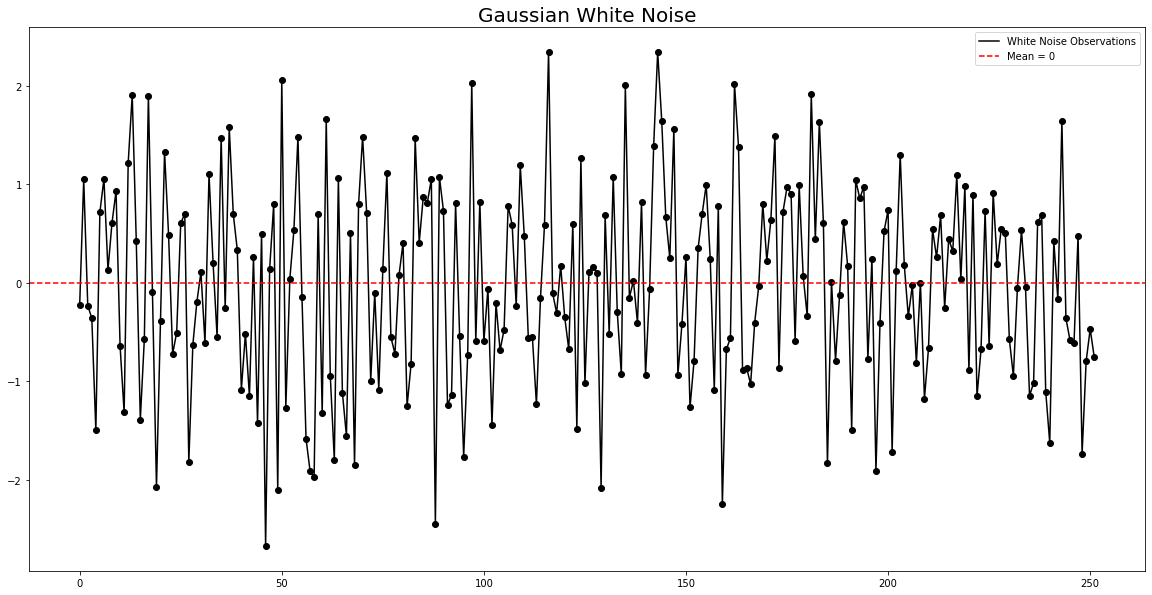
\includegraphics[scale=0.35]{images/GaussianWN.png}
\caption{Random Gaussian White Noise Example}
\label{fig: Gaussian WN}
\end{figure}

\subsection{Properties Financial Data}
Unique to financial data, specifically continuous stock returns, there are properties or "stylized facts" \cite{Popov2022} that are used as a guide.   

\begin{enumerate}
    \item The distribution of the returns are non-normal in two ways:
    \begin{enumerate}
        \item More mass in the tails (fat tails) - greater probability of events further from the mean
        \item There is a higher peak than a normal distribution (leptokurtic) - greater clusters of data at the mean
    \end{enumerate}
    \item Raw returns are uncorrelated, but transforming to squared or absolute, significant autocorrelation is observed
    \item "Volatility Clustering" - if today's return has a large absolute value it tends to be followed by another return with large absolute value, and visa versa with smaller values oof returns.  
\end{enumerate}

\cite{Popov2022}

\section{Motivating Example}
The properties of volatility when modelling returns guide us to the types of models we are using. For example, take Lloyds Banking Group, PLC (LLOY.L)'s returns from 2017 - 2020. Using Maximum Likelihood Estimation, I fit the log returns to a distribution and found they fit best to a Cauchy distribution with a location parameter -0.108 and Scale: 0.76 $\mathbf{Figure 1.2}$. If I assumed mean and volatility to be constant, its expected value is shown by the bottom plot in $\mathbf{Figure 1.3}$. Intuitively this is illogical, financial time series data are dependent on its location in the series, not random observation, this series assumes complete randomness with fat tails that are causing great changes. Comparing the red line in 1.3 to the true Lloyd's returns in the blue line, it is clear the observations volatility's are clustered and the tails are larger than a normal distribution. 
\begin{figure}[H]
\centering
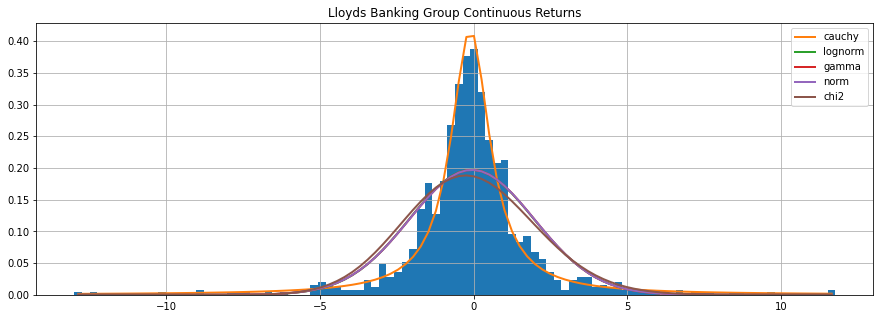
\includegraphics[scale=0.45]{images/LLoyReturnsDistribution.png}
\caption{Lloyds Returns Fitted Distribution}
\label{fig: LLOY Fitted Distribution}
\end{figure}
\begin{figure}[H]
\centering
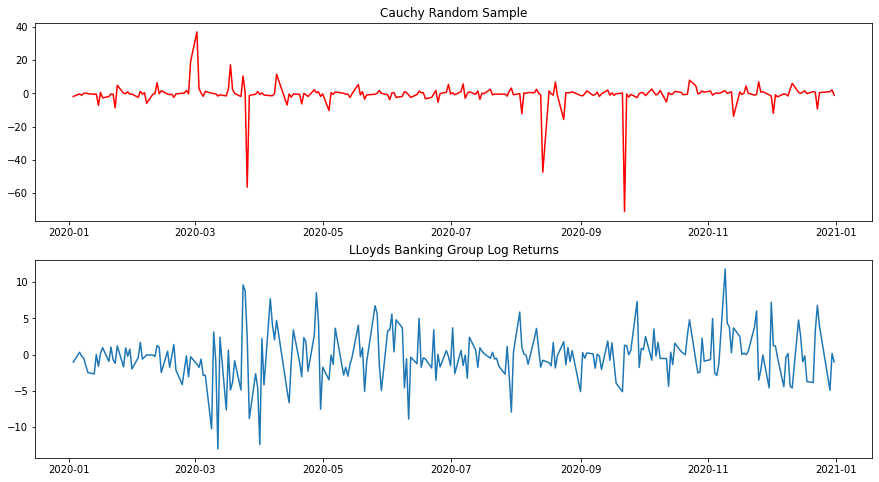
\includegraphics[scale=0.45]{images/LLOYvsCauchy.png}
\caption{Lloyd's Returns vs Cauchy Simulated Returns}
\label{fig: Returns v Cauchy}
\end{figure}
Therefore, this dissertation seeks to find a more accurate and efficient way to model stock market returns to extract the volatility/instantaneous standard deviation.  
\section{Irithmics Exogenous Data}

In an attempt to approach this problem from a novel direction, I will incorporate an exogenous variable into the volatility forecasting model with the hope of increasing the predictive power. Graciously, Irithmics, a U.K. based financial technology and data company donated data it's deep learning machine generated. These data include over a 170 trading days, each with 75-80 a probability density function indexed on each day with the probability value of how likely the deep learning algorithm believes an aggregated group of 250,000 funds will sell/short a specific stock. The corporation's method: 
"Our platform uses state-of-the-art deep learning originally designed to help describe and understand the spread and impact of long-term chronic human diseases, like diabetes. We have applied these technologies to learn from over 250,000 global institutional investors and funds, across hundreds of thousands of portfolios with a combined value of many trillions of dollars" \cite{Irithmics}. The compelling aspect of this exogenous data is it is not objectively correct and therefore the model contains many layers of uncertainty. First, there is the challenge of accurately estimating parameters and hyper parameters, as well as model selection, then whether or not Irithmic's algorithm during the selected time period is an accurate representation of the investors future behavior, and finally if the accurate prediction of the institutions behavior has any significant effect on the volatility of a certain stock's returns. Not only does this problem incorporate the concept of "The Wisdom of Crowds" but also the "Crowd" relationship with stock return volatility.

\section{Data Selection}
\subsection{2020}
There was unprecedented amounts of uncertainty and stock market volatility in 2020 due to the COVID-19 Pandemic. While this was a somber time for humanity, it gives the opportunity to stress test models and model accuracy during extremely uncertain points in time. Generally, forecasting is easy during stable and predictable points in time, but money is made and lost during times where no one knows what to do.  
\subsubsection{FTSE 100}
 Specifically, This analysis will be done on four FTSE 100 Companies from 4 different sectors. The FTSE 100 is the Financial Times Stock Exchange is the largest 100 companies listed in the United Kingdom by market capitalization. I will chose one from: \begin{itemize}
    \item Banking/Finance - LLoyds Banking Group
    \item Technology Vodafone
    \item Automotive - Rolls Royce
    \item Consumer Goods - Tesco
\end{itemize}

\subsection{Forecasting}
Unlike predictions, which rely on a set of non time indexed inputs, forecasting a time series requires always looking forward in time. This poses a larger challenge as fitting, training, and testing models must only focus on predicting out of sample data that lies forward in time. This research will specifically be focused on what is called "nowcasting". The phrase comes from the study of meteorology where weather events are forecast in very near future. The concept will be applied to stock market returns to forecast volatility for what is called a 1 day ahead rolling forecast. 

\section{Wisdom of the Crowds}
\subsection{Book}
In 2004 James Surowiecki, a staff writer at the New Yorker, wrote the book: "The Wisdom of Crowds: Why the Many Are Smarter Than the Few and How Collective Wisdom Shapes Business, Economies, Societies and Nations". The book spoke on his belief that effective and accurate decision making can almost always be improved by aggregating individual forecasts/predictions/decisions rather than individuals making decisions on their own. The simplest example from the book was the old story about Sir Francis Galton, being taken back at a silly carnival game for a crowd to guess the weight of an ox. The mean of the guesses was accurate, while the individual guesses themselves were no good. This is what the wisdom of the crowds or aggregation of the crowd intellegence. This isnt a statistical text, but gives an idea into how the concept of forecast aggregation and crowd wisdom can play into this research paper. The irithmics data aggregates their perceived action from the crowd. On day X, there is a Y\% chance that the 250,000 funds surveyed will short stock Z. If they are shorting stock Z, they are hoping that the stock will go down as they are in the business of making money of their trades. So, the question now becomes, are the crowds wise? are the fund managers aggregated forecasts better than picking say, one fund at Bridgewater Associates, one trader at Jane Street? This paper hopes to incorporate that information, not for stock prices, but to help with the predictions of volatility within the volatilty forecasts.   

The book also acknowledges that all group forecasts aren't created equal. To identify a "wise" crowd there must be: 
\say{\begin{enumerate}
    \item Diversity of Opinion
    \item Independence
    \item Decentralization
    \item Aggregation 
    \item Trust
\end{enumerate}
}\cite{wiki:crowds} 
These ideas for using crowd sourced things can be useful in statistical context, each of these items can be good steps for proper data sampling.   

Conversely, there are some integral failures of the crowd. These intuitively are the inverse of a smart crowd: 
\say{
\begin{enumerate}
    \item Homogeneity
    \item Centralization 
    \item Division
    \item Imitation
    \item Emotionality
\end{enumerate}
} \cite{wiki:crowds} The idea would to be cognizant of the data sampled and the derived forecast one would use. This comes back to the garbage in garbage out modelling, where the data is the most important piece of modelling. One would want to obtain varying forecasts to aggregate from every sense of varying. Socioeconomic Status, , Demographics location time etc etc spatial temporal. 
\subsection{Application}
The compelling aspect is a form of forecast aggregation has already happened and this project seeks extend the aggregation further. The difference is there is also a question of whether or not the forecast itself carries any relevance in the topic. Irithmics aggregated their machine's deep learning prediction on when the aggregation of funds will sell a stock, but is this relevant to the volatility and can this aggregation be aggregated with the empirical forecast. 

\chapter{Literature Review}


\section{Volatility Modeling of Stocks from Selected Sectors of the Indian Economy Using GARCH}
\subsection{Overview}
\cite{9544977} is a recent paper presented at the 2021 Asian Conference on Innovation in Technology (ASIANCON). This paper visits the idea of volatility clustering applied to the Indian Economy and therefore on Indian stocks on the NSE. The paper focuses on applying only the concept of \textbf{GARCH} or Generalised AutoRegressive Conditional Heteroscedasticity models to forecast volatility of returns rather than incorporating any exogenous variables or data.
\subsection{Methodology}
As the models the researchers considered were quite straightforward and easy to implement in Python, they took a very structured approach to the problem by beginning with the most simple \textbf{GARCH(1,1)} model, and then added complexity. This meant beginning with a constant mean model and normally distributed residuals, followed by skewed -t distributed resiudals. They then fit an Autoregressive Moving Average mean model residuals into the model and took the minimum AIC. Then they fit Asymmetric volatility models on the return series, this for example is the \textbf{GJR-GARCH} and \textbf{EGARCH} models which asses the impact of a negative shock as more impactful than a positive one. 
\subsection{Results}
The results were completed by testing the best model by minimum AIC with some out of sample data that the model has not seen. They used an expanding window and fixed window forecast and backtested the \textbf{EGARCH} Model. This was evaluated by a lot of different statistics on the Auto and Banking Sector and \textbf{EGARCH} in this scenario was best chosen.
\section{An Empirical Study of Hang Seng Index Based on GARCH Model}
\subsection{Overview}
\cite{LR2} is a recent paper presented at the 2020 second international conference on Economic Management and Model Engineering (ICEMME). The aim was to give an overview of optimal model fitting on the Hang Sang Index. The HSK is 33 stocks, akin to FTSE100, that look to give an overview of the economic and financial activity and health of the honk kong markets. The power of this index is it includes mainland china based companies in addition to Hong Kong. As discussed, the paper admits that the volatility of stock market returns are time-variant and therefore traditional measurements of standard deviation of the whole sample are useless. The goal of this paper was to evaulate what variant of a \textbf{GARCH(p,q)} model would fit best to the data
\subsection{Methodology}
Contrary to R's rugarch, or Python's arch library the researchers used Eviews10 software accompanied by the stock market data provided by the Flush Database. The returns calculated were log or continuous returns ($r_t = ln(P_t)-ln(P_{t-1})$). They did exploratory analysis on the data and determined it was stationary, and it was correlated enough to continue their analysis. To select the model they fit \textbf{GARCH(1,1)}, \textbf{GARCH(2,1)}, \textbf{GARCH(1,2)}, \textbf{GARCH(2,2)} and picked the best model from the Akaike Information Criteria or AIC. Using minimum AIC they chose the \textbf{GARCH(1,2)}. 

\subsection{Results}
The main takeaways the researchers had from this analysis were that the continuous returns (log change in daily prices) of the Hang Seng Index did have volatility clustering. The returns also had from the stylized facts fatter tails and sharper peaks in the distribution (similar to $\mathbf{Figure~1.2}$). They also determined there were no unit roots in the returns sequence, therefore inferred signs for stability, while through analysis of autocorrelation there was no monthly correlation. The drawbacks were the lack of sample size, but found as usual that the \textbf{GARCH} model's Variance predictions were very adequate for stock market returns. 

\section{A GARCH approach to model short-term interest rates: Evidence from Spanish economy}
\subsection{Overview}
\cite{https://doi-org.ezproxy.st-andrews.ac.uk/10.1002/ijfe.2234} was published in September 2020 in the International Journal of Finance and Economics. Instead of talking about stock market returns, this paper gives a derivative approach, modelling short term interest rates of three year Spanish government issued bonds. Again, this process is completed because the researcher believes that \textbf{GARCH} models provide: "a valuable alternative against econometric specifications that imply a homoscedastic error term" \cite{https://doi-org.ezproxy.st-andrews.ac.uk/10.1002/ijfe.2234}. The data is taken from January 1995 to December 2000 and is useful as there will be exogenous volatility caused by what they say is the European Central Bank assuming monetary sovereignty. 
\subsection{Methodology}
The paper takes into account interest rate theory and the exogenous factors that affect the rate that money is returned as a profit for the buyer of the bond, there is expectations, liquidity preference, institutional approach, habitat hypothesis, market segmentation hypotheses \cite{https://doi-org.ezproxy.st-andrews.ac.uk/10.1002/ijfe.2234}. They then applied a mathematical eiquation to the problem through the fisher information equation $$i_R = i_N -\pi$$ This effectively is the real interest rate is equal to the nominal interest rate minus the expected inflation rate. With this information they fit a \textbf{GARCH} model with the interest rates as the input hoping to obtain the conditional volatility of the time series
\subsection{Results}
The researchers found that this method of estimating the interests rates when breaking the traditional assumption of homoscedastic variance, instead with the heteroscedastic that \textbf{GARCH} employs was much more efficient and accurate. This model was more flexible as well, but a sub-specification of the \textbf{GARCH} model worked better than fitting through the traditional equation. The fisher equation was effective in its estimation of the government debt and they believe this can be expanded into other fields of finance and econometrics as well. \cite{https://doi-org.ezproxy.st-andrews.ac.uk/10.1002/ijfe.2234}
\chapter{Volatility Modelling Foundations}

\section{The ARCH \& GARCH Processes}
Because the aim of this research is to create, train and forecast accurate time series models, they must first be adequately introduced. As illustrated and explained earlier, returns of stock prices are non-linear in nature, stochastic processes, and have time variant instantaneous standard deviations/volatility. Because of this researchers have developed rigorous methods  to model these properties. 

\subsection{Foundations}
\subsubsection{Robert Engle}
In the 50th volume of the Econometrica Journal published in July 1982, Robert F. Engle introduced a paper titled "Autoregressive Conditional Heteroscedasticity with Estimates of the Variance of United Kingdom Inflation". This groundbreaking piece of work was extremely influential in leading the change in volatility modelling in econometrics. According to semantic scholar, the paper has been cited 19,974 times! On the 8th of October 2003, The Royal Swedish Academy of Sciences awarded Engle the Bank of Sweden Price in Economic Sciences in Memory of Alfred Nobel. They expalined: "He found that the concept of autoregressive conditional heteroskedasticity (ARCH) accurately captures the properties of many time series and developed methods for statistical modeling of time-varying volatility. His ARCH models have become indispensable tools not only for researchers, but also for analysts on financial markets, who use them in asset pricing and in evaluating portfolio risk" \cite{pressrelease_2003}. The paper introduced the concept that: " these are mean zero, serially uncorrelated processes with nonconstant variances conditional on the past, but constant unconditional variances. For such processes, the recent past gives information about the one-period forecast variance" \cite{engleOriginal}. 

\subsubsection{Tim Bollerslev}
In 1986 Tim Bollerslev took Engles ARCH Model one step further by creating a Generalized ARCH or GARCH Model. In his paper "Generalization of ARCH process" \cite{BOLLERSLEV1986307} he seeks to create a "more general class of process, GARCH, ... , allowing for a much more flexible lag structure" \cite{BOLLERSLEV1986307}. He took an imperical example of modelling inflation, by extending one of Engles papers from 1983's example. He compared his model, GARCH(1,1) with an ARCH(8) and found that: "In this light it seems that not only does the GARCH(1,1)model provide a slightly better fit than the ARCH(8) model in Engle and Kraft (1983), but it also exhibits a more reasonable lag structure" \cite{BOLLERSLEV1986307}. Fundamentally, the model extension lead to great gains and found that the research was able to be better explained using GARCH. 

\subsection{Mathematics \& Interpretation}
\subsubsection{ARCH}
The Autoregressive Conditional Heteroscedasticity "ARCH" model introduced by Engle considers the volatility or instantaneous standard deviation of a time series independent from its mean function and implied by the name, that volatility is time variant \cite{carmona2004}. The model takes one parameter as an input and is generally written as $\mathbf{ARCH(P)}$ . The volatility at time point $\mathbf{t}$ is calculated by considering $\mathbf{p}$ time periods in the past's value of the series multiplied by some parameter $\alpha_1$ plus another intercept parameter $\alpha_0$.$$\{X_t\}_t \sim ARCH(p) \iff X_t = \sigma_tW_t$$This function implies that $W_t$ is white noise and $\sigma_t$ is a positive function of the previous $\mathbf{p}$ lags (observations in the time series) \cite{carmona2004}. For example, the function to calculate the standard deviation for an $\mathbf{ARCH(1)}$ process is as follows: 
$$\sigma_t^2 = \alpha_0 + \sum^p_{j=1} \alpha_jX^2_{t-j}; ~ for~j = 1,2,...p$$This is not to say the only time period considered is p-behind, interestingly, the $\sigma_t$ is actually calculated as a weight decaying function of all of the previous lags in the time series, an infinite decay so to speak. 
$$ 
\sigma_t = \sqrt{\alpha_0(\sum^\infty_{j=0} \alpha_1^jW^2_{t-1}W^2_{t-2}...W^2_{t-j})}
$$Intuitively this explains the auto regressive nature that the current position relies on all the previous lags with decaying levels of importance, where $W^2_{t-1}$ is of greatest weight.

To intuitively understand the model, I find it best to consider a causal diagram of what actually affects the time series at $\mathbf{t}$. For an $\mathbf{ARCH(p)}$ process, 
$$
\xymatrix{
{X_t} \ar[dr] \ar[r] &\mathbb{\epsilon_t} \\
& \sigma_t \ar[r] & \hat{X}_{t-1}}
$$
Value of the time series at time point $\mathbf{t}$ t is calculated by white noise, multiplied by the square root of a constant, $\alpha_0$, plus a constant $\alpha_1$ multiplied by the value ofs time series squared: $\mathbf{\sigma_t\epsilon_t}$. As the diagram shows, the value of the time series, today, is affected by the random error $\epsilon_t$ today, as well as the volatility today. But, since the volatility is a function of the time series yesterday, we see that $\sigma_t$ is a function of $\sigma_{t-1}$. The autog regressive nature of the model, is simply an extension of the thought that $\sigma_t$ is a function of $\sigma_{t-1}$ because $\sigma_{t-1}$ is a function of $\sigma_{t-2}$ and so on and so forth. The weight of $\sigma_{t-n}$ to $\sigma_{t}$ depends on $\mathbf{|t-n|}$  \cite{GARCHYoutube}.

ARCH models are thought of as being "bursty" since, from the causal diagram the observation at time point t in the series is dependent only on the last value of the time series it can yield high peaks but values that are not sustained. The idea of volatility clustering is not modelled as well as it could, as the model would identify the peak to the new level of the cluster, but not for 3,5,7 days for example of sustained volatility \cite{GARCHYoutube}

\subsubsection{GARCH}

The GARCH model by nature is just an extension of the $\mathbf{ARCH}$ with a $G$. $G$ stands for Generalized and thus $\mathbf{GARCH}$ has a parameter $\mathbf{p}$ but also a second $\mathbf{q}$ ie $\mathbf{GARCH(p,q)}$. 

$$\{X_t\}_t \sim GARCH(p,q) \iff X_t = \mu_t+\sigma_tW_t$$

The distinct difference with the $\mathbf{GARCH}$ model is that the white noise is Gaussian. The new equation for $\sigma^2_t$ the instantaneous or current volatility at the time point now is $$\sigma_t^2 = \sigma^2 + \sum^p_{j=1} \phi_j\sigma^2_{t-j}+ \sum^q_{j=1} \theta_j\hat{X}^2_{t-j}; ~ for~j = 1,2,...p$$  
$$\mathbf{GARCH(1,1) ~~ : ~~~ }\sigma^2_t = \sigma^2 +\phi_1\sigma^2_{t-1}+\theta_1\hat{X}^2_{t-1}$$\cite{carmona2004}. Akin to ARCH, the model relies on the last $\mathbf{p}$ observation's value in the time series, but also the last $\mathbf{q}$ standard deviations. 
For $\mathbf{GARCH}$, since there is an extra dependency for $\mathbf{GARCH(p,q)}$ not just $\mathbf{ARCH(p)}$, the causal diagram has another element!
For a $\mathbf{GARCH(p,q)}$ process: 
$$
\xymatrix{
{X_t} \ar[dr] \ar[r] &\mathbb{\epsilon_t} \\
 & \sigma_t \ar[d] \ar[r] &\mathbb\hat{X}{_{t-1}} \\
 & \sigma_{t-1}}
$$
In the $\mathbf{GARCH}$ case, the value of the time series at time point $\mathbf{t}$, is calcualted the same way $\mathbf{ARCH}$ is, but now not only is the volatility, at time point $\mathbf{t}$ a function of the time series $\hat{X}_{t-1}$ yesterday, but it is also a function of the volatility $\sigma_{t-1}$ yesterday hence the two arrows coming from $\sigma_t$\cite{GARCHYoutube}.

Compared to ARCH the GARCH model lends itself to be better at modelling the volatility clusters. The model equation now shows that $\sigma_t$ the immediate or instantaneous volatility is a function of not only the last value of the time series but also the last value of the standard deviation. 

\subsubsection{Further Extensions}

The traditional $\mathbf{GARCH}$ model is the typical symmetric model that generally is used as it is extremely powerful and accurate, but over the years since Bollserslev proposed the paper there have been different derivative models. Discussed now are univariate models, where it takes one input, in this case log/continuous returns. There are also different models such as Exponential $\mathbf{GARCH}$ $\mathbf{(EGARCH)}$ Asymmetric $\mathbf{(GARCH)}$ $\mathbf{(AGARCH)}$, $\mathbf{GJR-GARCH}$, $\mathbf{TGARCH}$, $\mathbf{(APGARCH)}$, \textbf{GARCH}. These models derive different variances by modifying the generalized equation. For example, a very useful model, $\mathbf{(EGARCH)}$  the log of the variance instead of the variance for $\mathbf{(q)}$. \cite{GARCHMODels}

\section{Dynamic Conditional Correlation (DCC)}
To compare the volatility forecast from a univariate $\mathbf{GARCH(p,q)}$ model (modelling a single variable, continuous returns) with a multivariate model (two variables, continuous returns, Irithmics probabilities) I employed what is called a Dynamic Conditional Correlation "DCC" to evaluate the correlation. This model was again founded by the founder of the $\mathbf{ARCH(p)}$ model, Robert Engle. These models are said to be a "Simple Class" of multivariate GARCH models, but their strength is in its flexibility akin to a univariate GARCH process, while still a parameterized model. The models themsevles are not linear in nature, but do use maximum likelihood estimation and are empirically effective \cite{DCC}.   
The intuition behind this model is similar to that of the $\mathbf{ARCH/GARCH}$: Like volatility over time, the correlation between the volatilites of two time series' are not static, but instead dynamic and modelling them as an average over time instead of continuously dynamic is inadequate. Statically, conditional correlation between two observations is seen as:
$$ 
\rho_{1,2} = \frac{E_{t-1}(r_{1,t}r_{2_t})}{\sqrt{E_{t-1}(r_{1,t}^2r_{2_t}^2})}
$$
In order to transform this function into a dynamic and generalisable method, the company $RiskMetrics^{TM}$ has proposed using decaying weights through a $\lambda$ parameter. This has a drawback of an expanding window where correlations n periods behind are not being omitted, when they are clearly uninformative. The additional issue as found in many smoothing problems is there is no optimal parameter for $\lambda$, RM sets it equal to 0.94, but that is by no means optimal for all problems
$$
\hat{\rho}_{1,2} = \frac{\sum^{t-1}_{s=1}\lambda^{t-j-1}(r_{1,s}r_{2_s})}
{\sqrt{\sum^{t-1}_{s=1}\lambda^{t-j-1}(r_{1,s}^2r_{2_s}^2})}
$$

The way Engle remedied this impass was by using a "natural alternative" to exponential smoothing, by instead using the GARCH(1,1) model and incorporating the correlation estimator giving the covariance matrix: $Q_t = |q_{i,j,t}|$ which is " is a weighted average of a positive definite and a positive semidefinite matrix" \cite{DCC}. The mathematics is quite complicated, but it is easily implemented in Python. 

\section{GARCH with Exogenous Regressor}
In order to fit this exogenous covariate of Irithmics probabilities, the univariate $\mathbf{GARCH}$ model must be extended. The choice for this research was, using the probabilities themselves as an exogenous regressor. Letting the next out of sample regressor be equal to $\pi$, the multivariate $\mathbf{GARCH}$ model is:

$$
\sigma_t^2 = \sigma^2 + \sum^p_{j=1} \phi_j\sigma^2_{t-j}+ \sum^q_{j=1} \theta_j\hat{X}^2_{t-j} + \beta_0 + \beta_1[\pi_1,t] ; ~ for~j = 1,2,...p
$$
\chapter{Methodology}

\section{Data}
\subsection{Processing}
\subsubsection{Stock Returns}
To obtain stock market returns for Lloyd's, Tesco, Rolls Royce and Vodafone, I used Python 3.9 \cite{Python3} and the Pandas \cite{pandas} library to interact with the Yahoo Finance API. I was specifically working with the closing price (price at the end of the trading day) and the data span from the first trading day in 2017 to the last in 2020. To calculate continuous daily returns I used the formula:
$$
r_t = ln({close}_t) - ln({close}_{t-1})
$$
I chose the continuous daily returns instead of the discrete returns because of the mathematical ease of temporal aggregations for multi-period continuous returns are simply the sum of the logarithmic returns. Take for example k-periods: $r_t(k) = ln(P_t) - ln(P_{t-k})$. I chose to use a simple tool like the Yahoo Finance API over a real time data feed such as Refinitiv because I used simple closing prices of years prior historical stock market data. If I was planning analysis of high frequency time periods, I surely would have used it, but this was easier to implement to the models and has greater opportunity for repeatability by others as Yahoo Finance is free. 

\subsubsection{Irithmics Data}
Unlike simple closing prices of a stock, the data provided by Irithmics arrived in a much more complex way. These data were delivered in comma separated value (.csv) format, that for each company in the FTSE 100, and each trading day in 2020, included a derived discrete probability density, indexed with between 75 and 80 days, describing the probability the deep learning algorithm assigned of a short/sell by the group of funds. $\mathbf{Figure 4.1}$ contains a visual example of what the files for date index January, 26th look like. As this is akin to a probability density, the values on each day will sum to one. 

\begin{figure}[H]
\centering
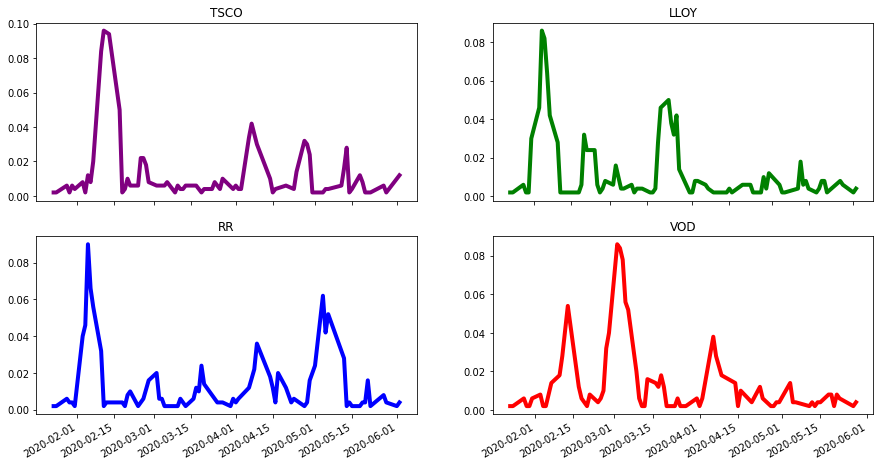
\includegraphics[scale = 0.45]{images/irithmicsprobs.png}
\caption{January 26th Irithmics Probabilities Example}
\label{fig: Irithmics Plot}
\end{figure}

\subsection{Exploratory Data Analysis}
\subsubsection{Stock Returns}


Before building and training any time series models, I first needed to understand and summarise the properties of each of the chosen companies continuous returns. This was guided by the properties of financial asset returns introduced in $\mathbf{Section~1.2.2}$. Because this research is directly focused on volatility, my first step was to obtain the sample standard deviation of each stock's returns, and plot it over the absolute value of those returns $\mathbf{Figure~4.2}$. I assessed the absolute value of the returns rather than the raw value for ease of visualization. The aim of these plots were to evaluate whether or not the returns showed signs of time varying volatility, and volatility clustering. It was immediately apparent that all four stock's returns visually displayed features of both. 

\begin{figure}[hbt!]

\begin{subfigure}{.49\linewidth}
  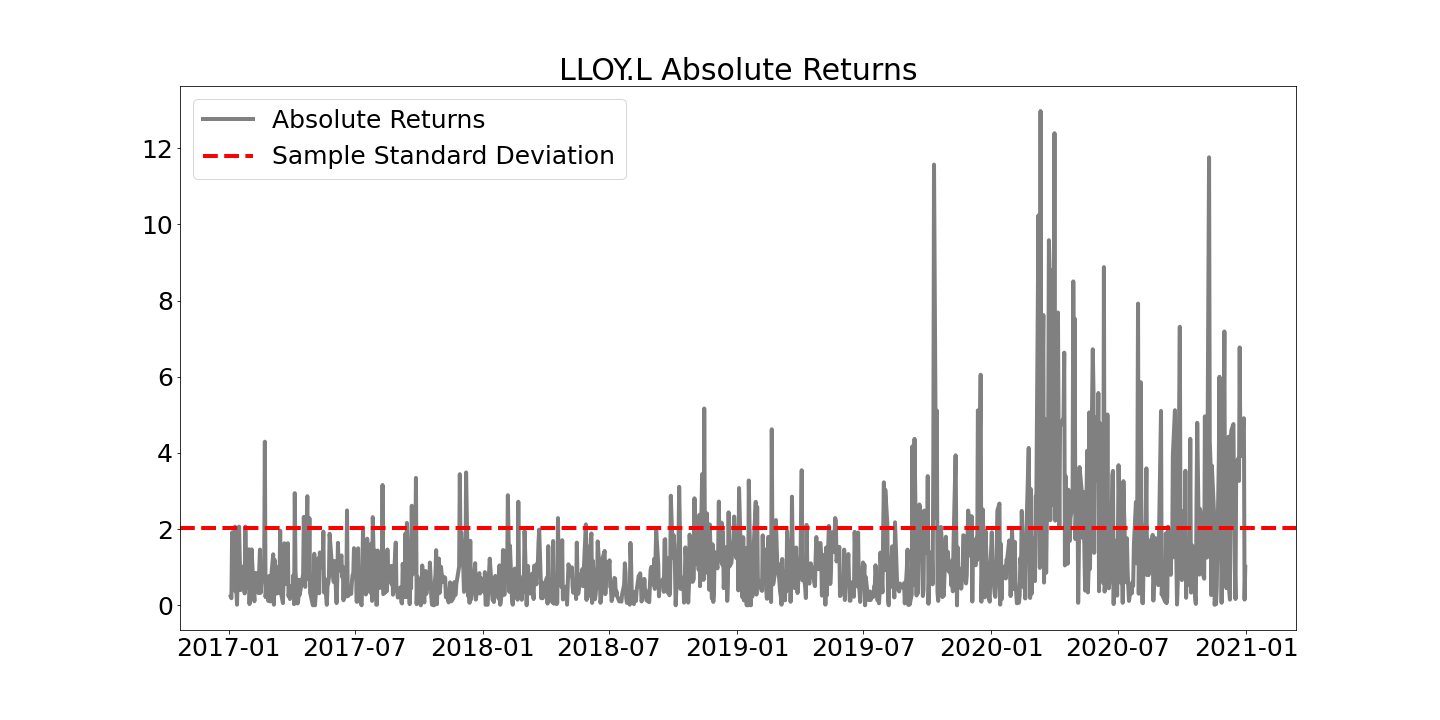
\includegraphics[width=\linewidth]{images/Exploratory/plot 1.png}
  \caption{LLOY}
  \label{A}
\end{subfigure} % <-- "\hfill"
\begin{subfigure}{.49\linewidth}
  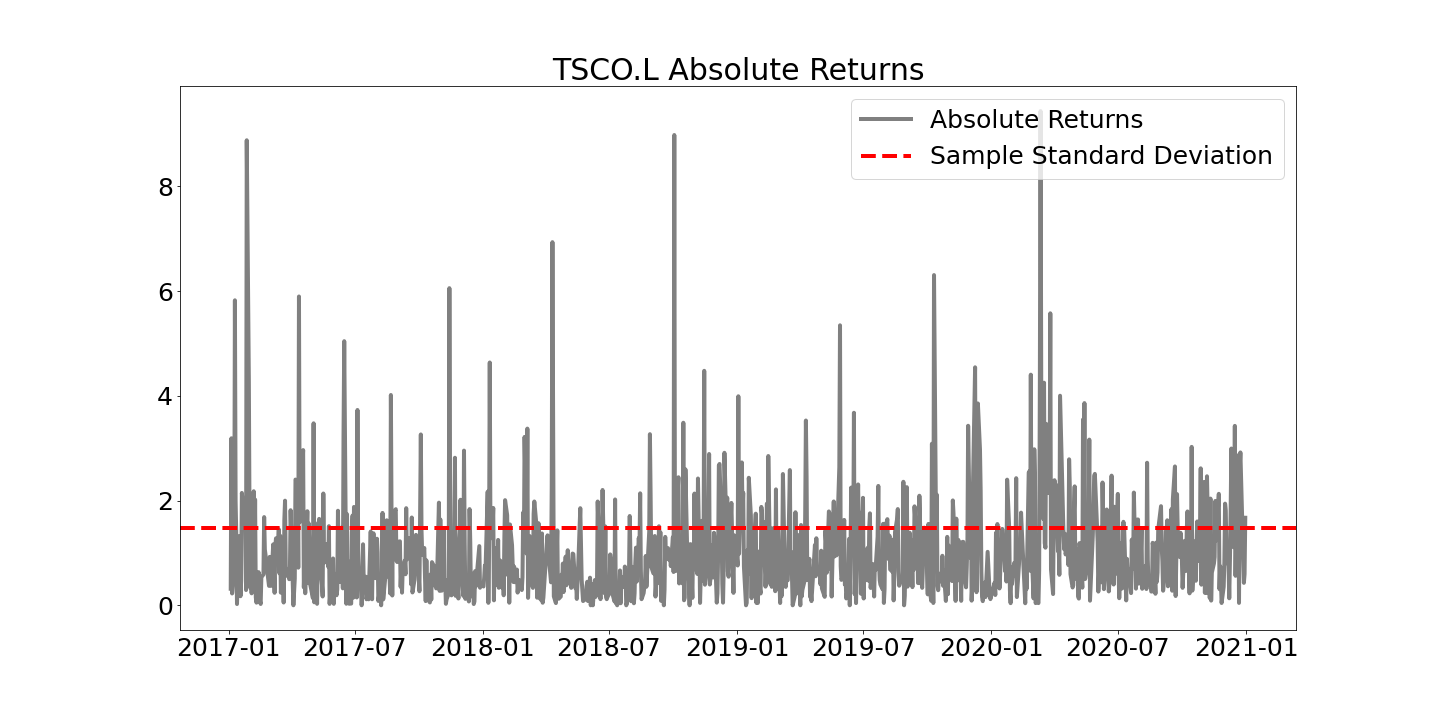
\includegraphics[width=\linewidth]{images/Exploratory/plot 2.png}
  \caption{TSCO}
  \label{B}
\end{subfigure}

\medskip % create some *vertical* separation between the graphs
\begin{subfigure}{.49\linewidth}
  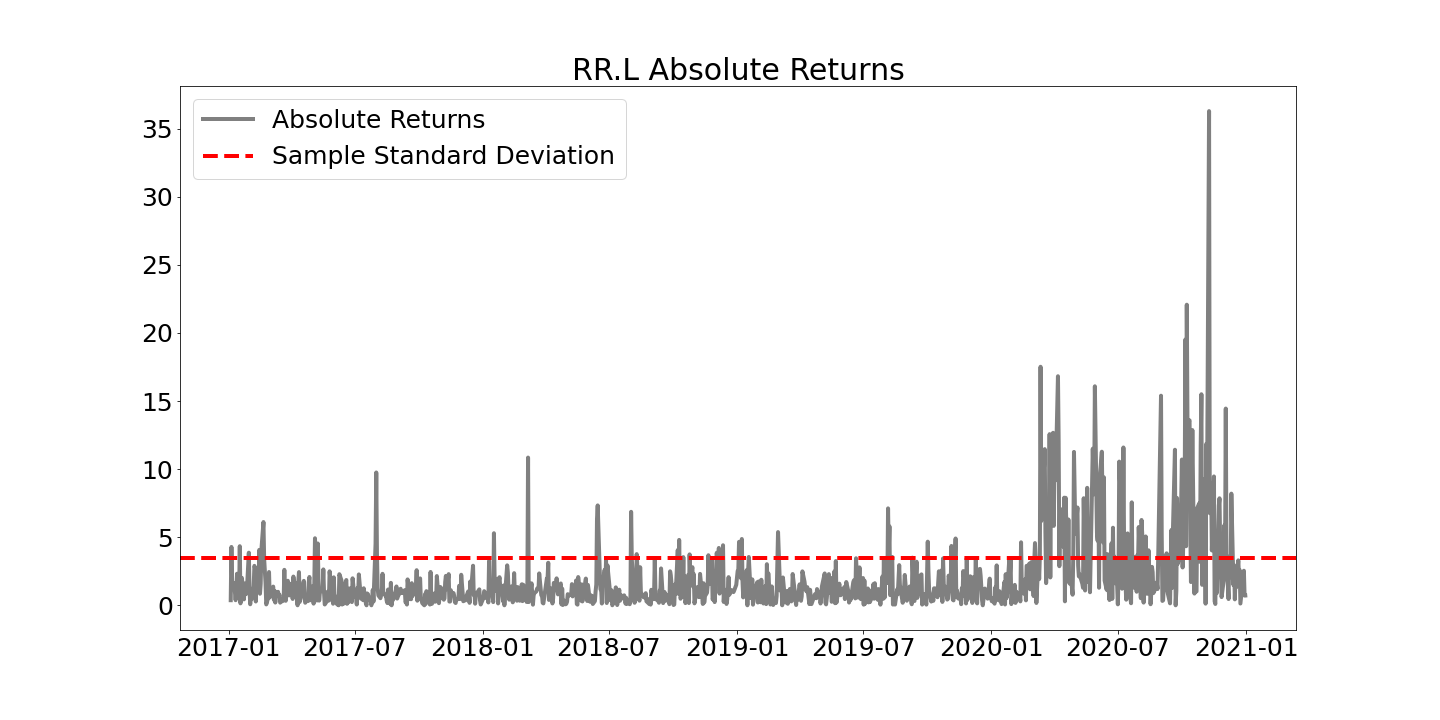
\includegraphics[width=\linewidth]{images/Exploratory/plot 3.png}
  \caption{RR}
  \label{C}
\end{subfigure} % <-- "\hfill"
\begin{subfigure}{.49\linewidth}
  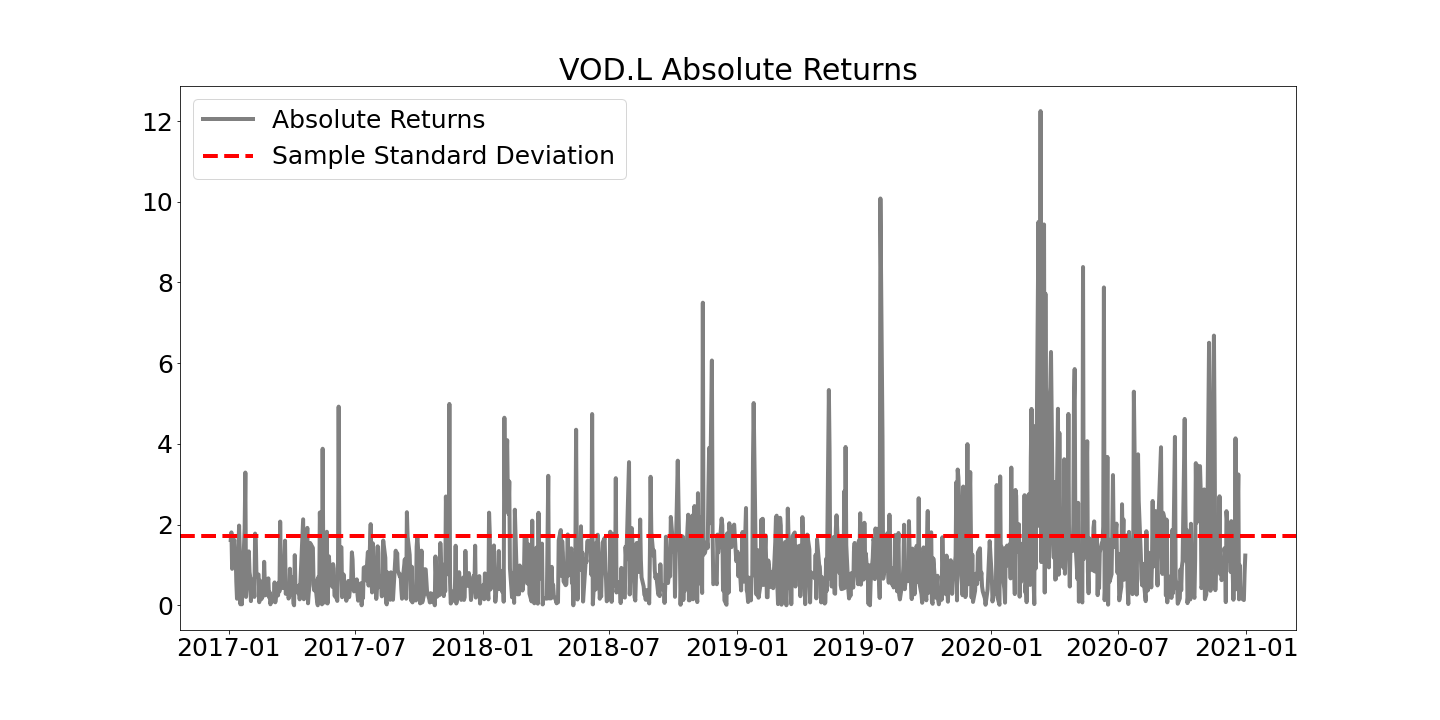
\includegraphics[width=\linewidth]{images/Exploratory/plot 4.png}
  \caption{VOD}
  \label{D}
\end{subfigure}
\caption{Returns v Sample Standard Deviation}
\end{figure}
The next step in exploration was to identify the distribution of the returns. The first and second properties explained that the distribution of the returns should show more probability mass in the tails, as well as having a higher peak than a normal distribution. I implemented $\mathbf{Figure~4.3}$ by using the 'Fitter' Python library. This library implements a kernel density estimation, histogram, as well as overlays other common distributions over the sample data. The distributions are fit using maximum likelihood estimation. Each of the four stocks exhibited the properties of distributions of asset returns differently, following different distributions. Nonetheless, the outcomes were all encouraging and prompted me to continue with the analysis. 

\begin{figure}[hbt!]

\begin{subfigure}{.49\linewidth}
  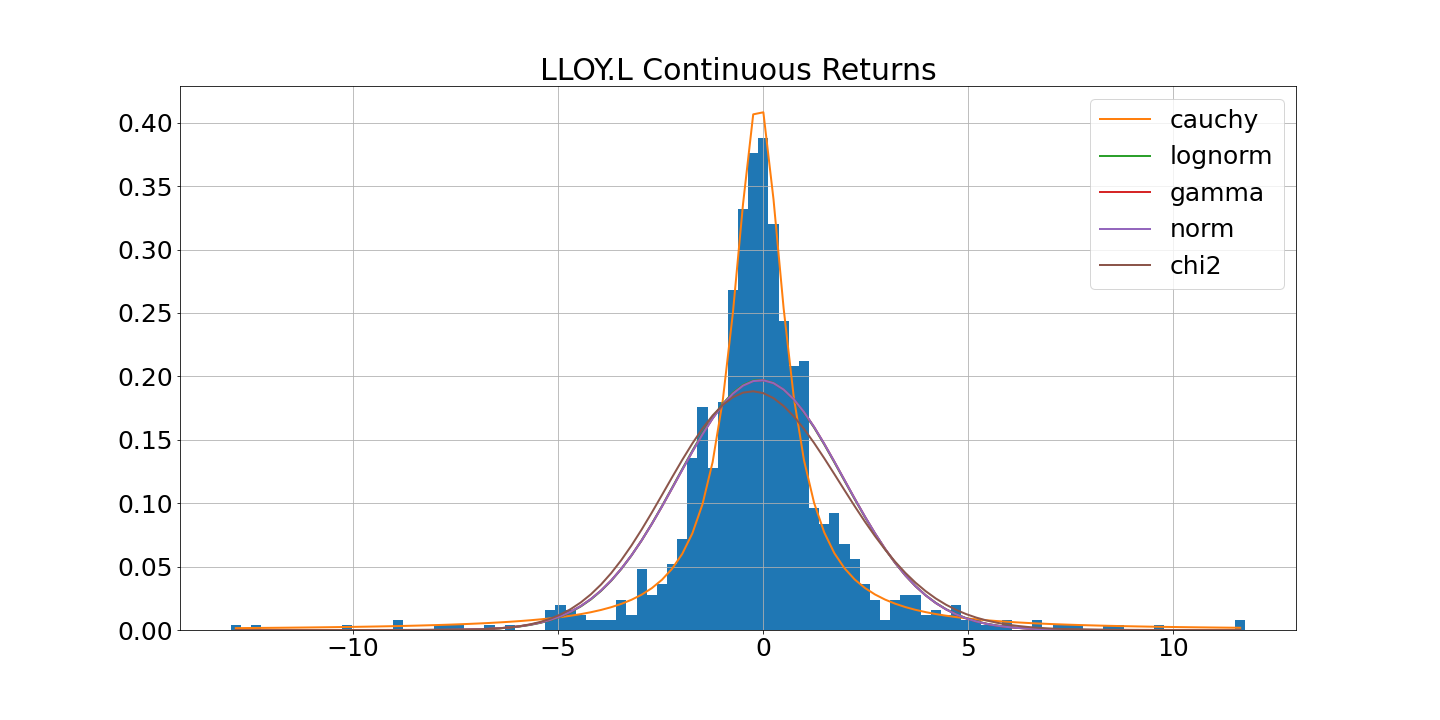
\includegraphics[width=\linewidth]{images/returnDist/plot 1.png}
  \caption{}
  \label{MLEDdet}
\end{subfigure} % <-- "\hfill"
\begin{subfigure}{.49\linewidth}
  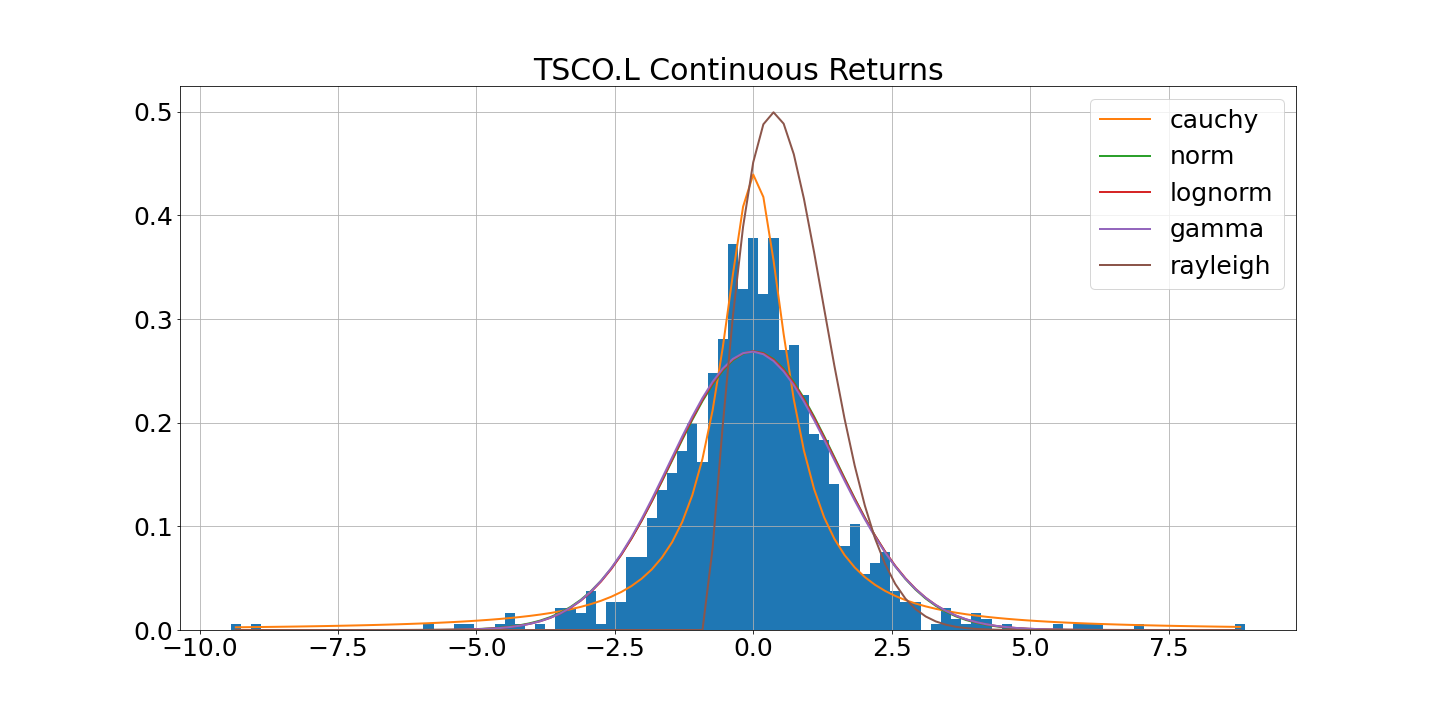
\includegraphics[width=\linewidth]{images/returnDist/plot 2.png}
  \caption{}
  \label{energydetPSK}
\end{subfigure}

\medskip % create some *vertical* separation between the graphs
\begin{subfigure}{.49\linewidth}
  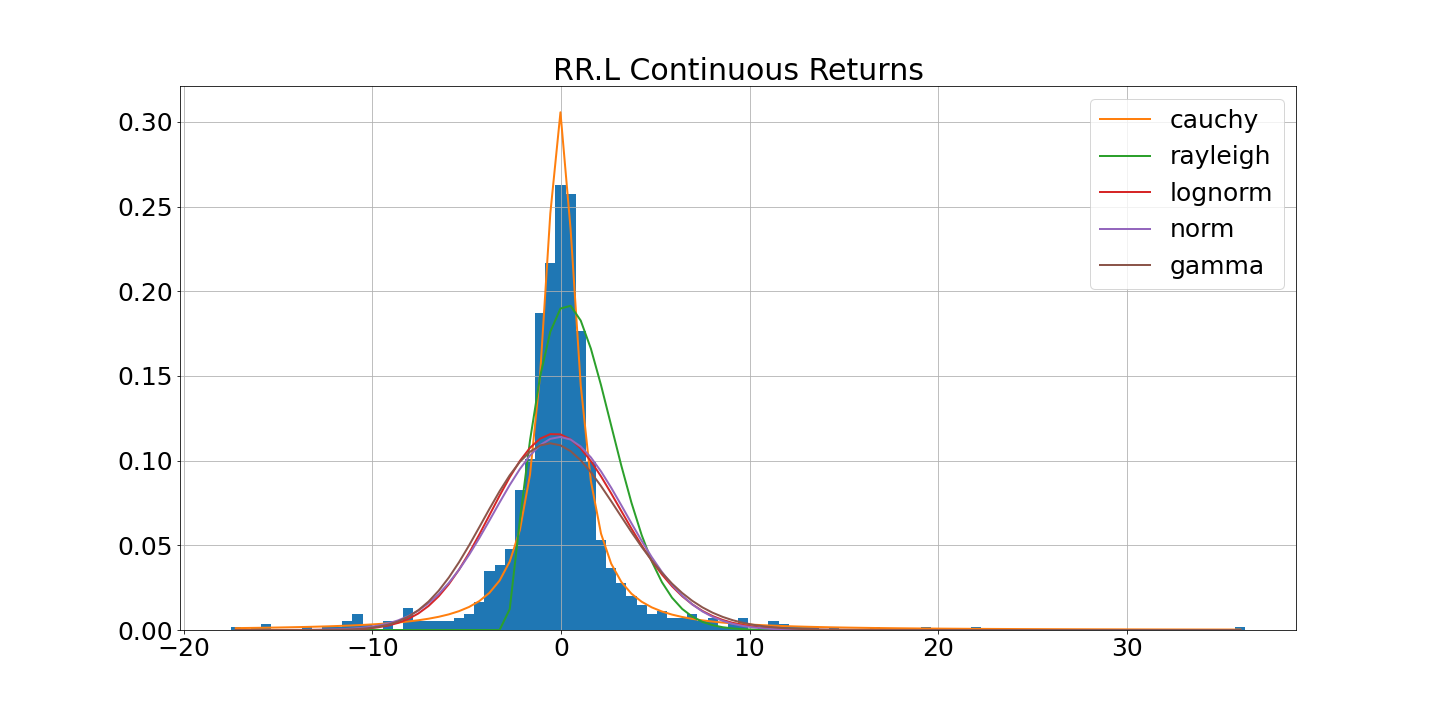
\includegraphics[width=\linewidth]{images/returnDist/plot 3.png}
  \caption{}
  \label{velcomp}
\end{subfigure} % <-- "\hfill"
\begin{subfigure}{.49\linewidth}
  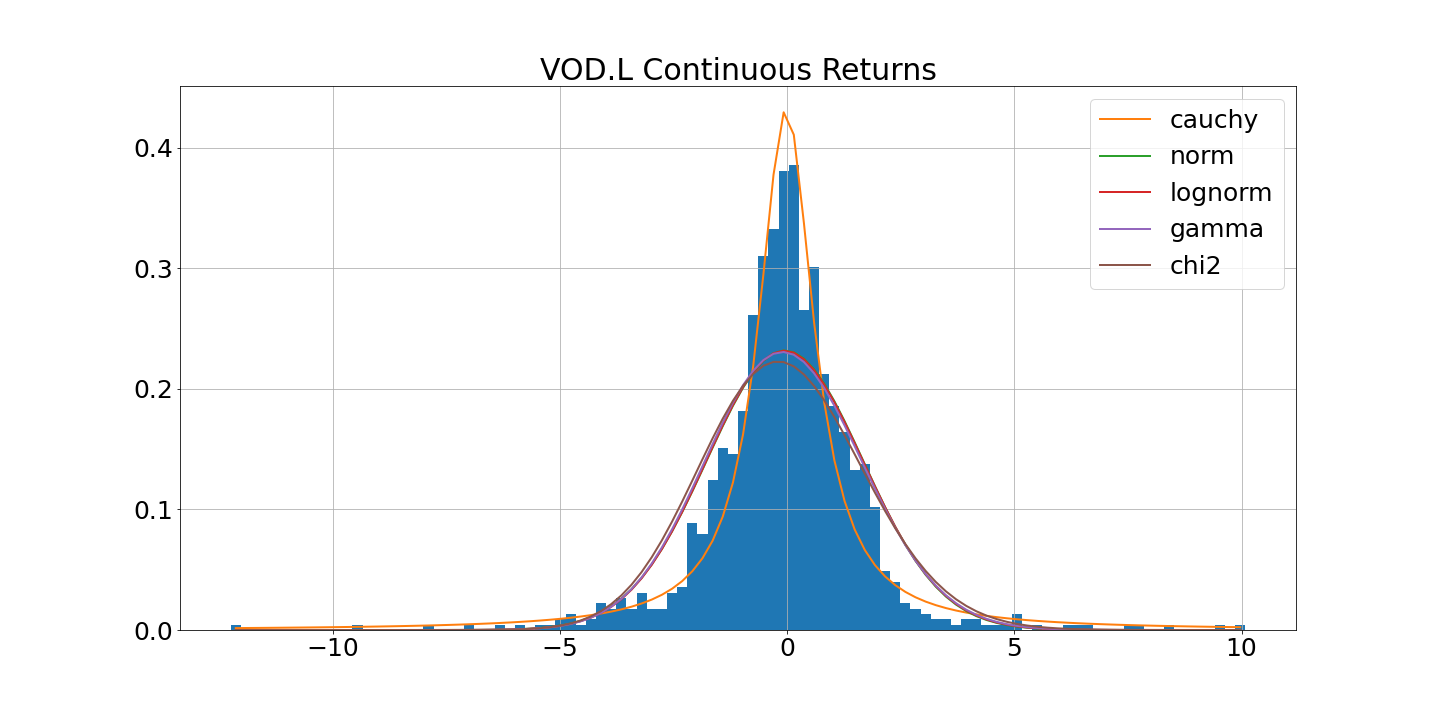
\includegraphics[width=\linewidth]{images/returnDist/plot 4.png}
  \caption{}
  \label{estcomp}
\end{subfigure}
\caption{Returns Distribution}
\end{figure}

The next step was to evaluate the third property of correlation. Since asset returns are said to have minimal to no autocorrelation in continuous returns, but significant autocorrelation in absolute or squared returns \cite{Popov2022}, I transformed the data into squared returns, and plotted the partial autocorrelation function outcome for Lloyd's as an example in $\mathbf{Figure~4.4}$. The plots visually displayed minimal to no autocorrelation between raw returns, but significant partial autocorrelation in squared returns. This is very important to see, as intutively, this is illustrating how, for example, the returns of a stock today, are significantly dependent on the returns of the past 1-3 days. For conditional volatility models such as $\mathbf{GARCH}$, this is of utmost necessity, as explained in $\mathbf{Section~3.2.2}$ the model depends on a specified number of days prior standard deviation and value in the time series. 
  
\begin{figure}[H]
\centering
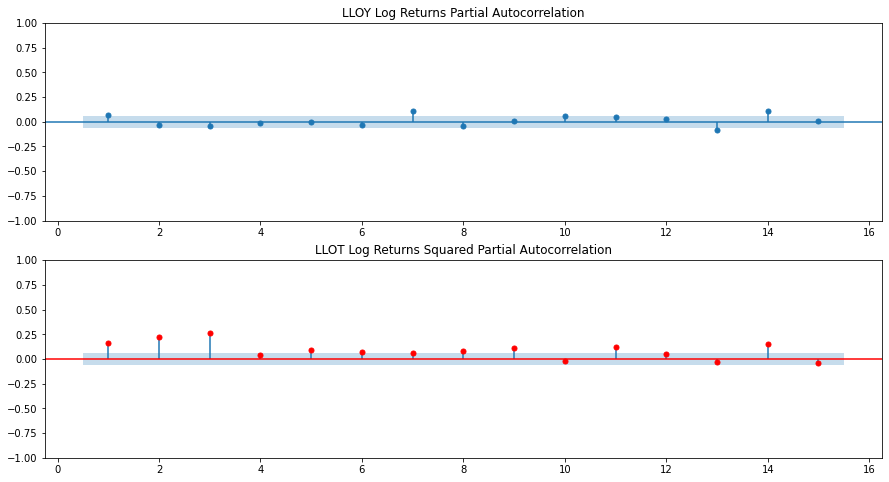
\includegraphics[scale=0.45]{images/PACF.png}
\caption{PACF: Normal v Squared Returns }
\label{fig: Returns v Squared}
\end{figure}

\subsubsection{Irithmics}
The exploration of Irithmics data posed a greater challenge. As these data are non-common and had no prior properties, a more creative approach had to be undertaken. For starters, I returned to $\mathbf{Figure~4.1}$, to get a sample visual representation of the properties of the data. It appeared there were signs of seasonality, or recurring external influences such as economic news or portfolio re-balancing. Something I had to take into great account when evaluating these data was trying not to over-fit models or ideas given the shape of one day's data. Each stock contained between 1-100 predictions for the same trading day, therefore keeping the analysis as generalisable as possible was paramount.    

Preprocessing these data posed two significant challenges: 1) generalisation, 2)formatting. As generalisation has already been discussed, the formatting issue needed to be remedied as fitting a conditional volatility model with an exogenous covariate works similarly to a regression model. The datasets have to be of the same length, and in time series the indices have to match. This meant I had to find a way to aggregate the already aggregated Irithmics probabilities, such that each stock only had one probability of short selling for each trading day. I completed this by implementing a weight decaying algorithm. This algorithm grouped the forecasts for each trading day (between 1-100 observations), and assigned a relative weight based on its temporal location. For example: the short/sell probability for March 25th has a prediction from all days January 1st - March 24th. To aggregate these forecasts, my goal was to mimic the concepts used in $\mathbf{GARCH}$ models, and transform the data into a single, univariate time series: the weight of the probabilities decayed based on its distance from the trading day, i.e. January 10th's prediction carries a lesser weight than March 10th's prediction for March 24th. The outcome of this algorithm is shown in $\mathbf{Figure~4.5}$ and the code can be found in the appendix. 


\begin{figure}[H]
\centering
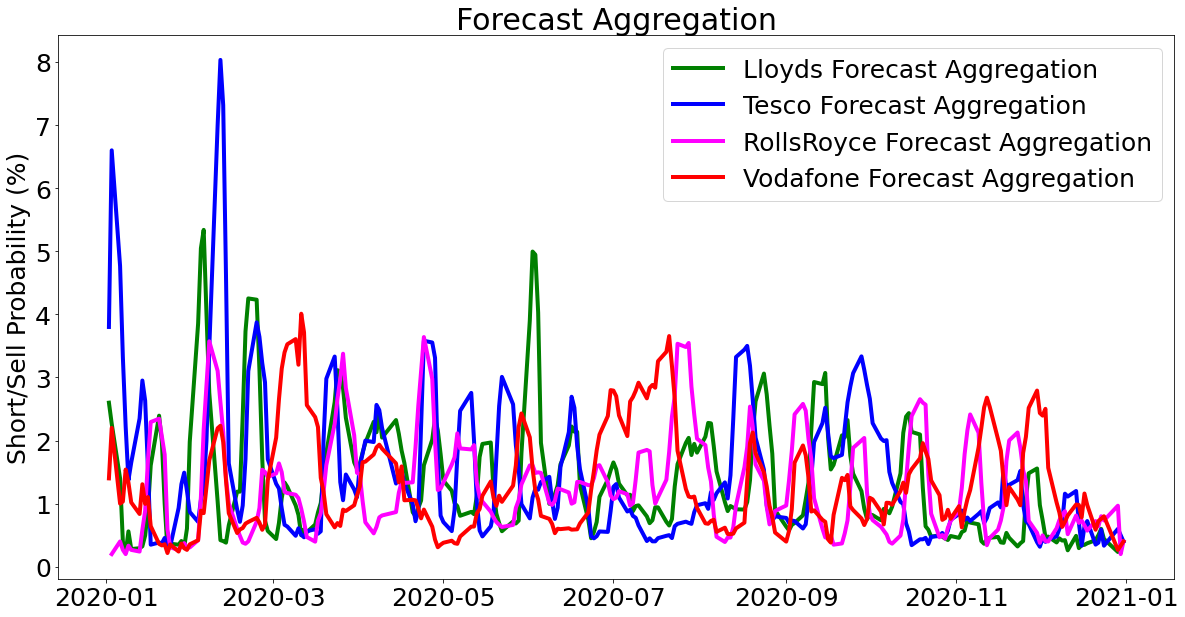
\includegraphics[scale=0.35]{images/Exploratory/forcAgg.png}
\caption{Irithmics Forecast Aggregation}
\label{fig: Irith Forecast Agg}
\end{figure}


\section{Model Fitting}
\subsection{Strategy}

When approaching the fitting and training of models I took a very structured approach. This was because each portion of the project directly built on the outcomes of the prior model. The necessity for consistency across univariate models and models with exogenous covariates cannot be understated as the comparison and impact of the addition of new information had to be the only change, otherwise there would be other factors affecting the forecasted values. The strategy was as follows:

\begin{enumerate}
    \item Implement grid search algorithm to search across combinations of parameters and hyper parameters
    \item Fit many models through algorithm for each stock without the exogenous covariate of Irithmics data
    \item Pick the best model based on Akaike Information Criterion (AIC)
    \item Fit a Dynamic Conditional Correlation (DCC) Model to GARCH Volaility and Irithmics Probabilities
    \item Fit the same model with an exogenous covariate
    \item Forecast last 25 trading days of 2020
    \item Compare generalisation error (MSE MAE)
\end{enumerate}

\subsection{Fitting}
Before I fit any models, I first created a holdout data set in order to retain, albeit small, very important out-of-sample (OOS) data. This data is important because the training and fitting of the models cannot be done with a dataset, and then predict already seen data. These models hopefully can be as generalised as possible, and when fed in new data for future events will have predictive accuracy. Since the sample size was quite small, only one year, the holdout or test data was 25 trading days, about the month of December, 2020. This data is interesting because in the United Kingdom at the time, there was great uncertainty around the next lockdown which inevitably came, and therefore had high potential for greater levels of volatility. 

\subsubsection{Univariate}
To search for the best model, I implemented a grid search algorithm in Python. A grid search's goal is to find optimal hyperparameters in a model, based on a specified loss function. In this case, the available hyperparameters were: Volatility (GARCH/EGARCH), the associated lags (p,q), and the residual distribution (students-t, skewed-t). The chosen loss function is the Akaike Information Criterion (AIC) which is calculated by $$ AIC~=~2(K) - 2ln(L)$$ where $\mathbf{K}$ is the number of parameters and $\mathbf{L}$ is the likelihood. This loss function penalises more complex models as I look to minimise the AIC value. Based on this specification, the algorithm fit 72 different univariate models and returned a list of the top five and bottom five combinations based on this criterion $\mathbf{(Figure~4.6)}$.
\begin{figure}[hbt!]
\begin{subfigure}{.49\linewidth}
  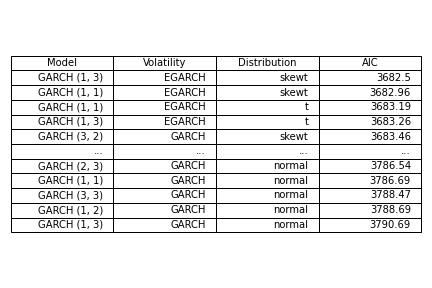
\includegraphics[width=\linewidth]{images/modelFit/stockLLOY.L.png}
  \caption{LLOY}
  \label{fig:A}
\end{subfigure} % <-- "\hfill"
\begin{subfigure}{.49\linewidth}
  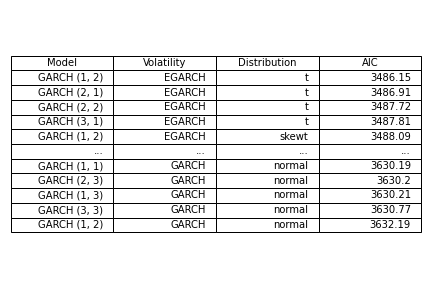
\includegraphics[width=\linewidth]{images/modelFit/stockTSCO.L.png}
  \caption{TSCO}
  \label{fig:B}
\end{subfigure}
\medskip % create some *vertical* separation between the graphs
\begin{subfigure}{.49\linewidth}
  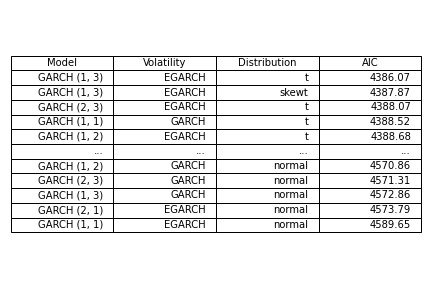
\includegraphics[width=\linewidth]{images/modelFit/stockRR.L.png}
  \caption{RR}
  \label{fig:C}
\end{subfigure} % <-- "\hfill"
\begin{subfigure}{.49\linewidth}
  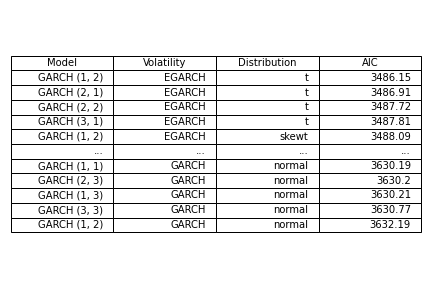
\includegraphics[width=\linewidth]{images/modelFit/stockTSCO.L.png}
  \caption{VOD}
  \label{fig:D}
\end{subfigure}
\caption{Grid Search}
\end{figure}

\subsubsection{Dynamic Conditional Correlation}
While the equations are quite complex, implementing this in Python was rather manageable. Though no available libraries, the researcher by the alias: \cite{DirtyQuant} implemented this in their own project, which I used as a guide. The model took the stock returns and Irithmics probabilities as input, runs a univariate $\mathbf{GARCH}$ model on each series to obtain a conditional volatility estimate, then takes the conditional volatilities as input, into the DCC equation. For each stock and probability pair, the output is a single series containing the Dynamic Conditional Correlation $\mathbf{Figure~4.7}$. The DCC gives information on the dynamic relationship between the two variables, and I hoped to see greater correlation in times of high volatility, which would prompt the model to have an increase in forecast accuracy since I will be fitting the Irithmics data as an exogenous regressor, a linear relationship would show itself here. 

\begin{figure}[H]
\centering
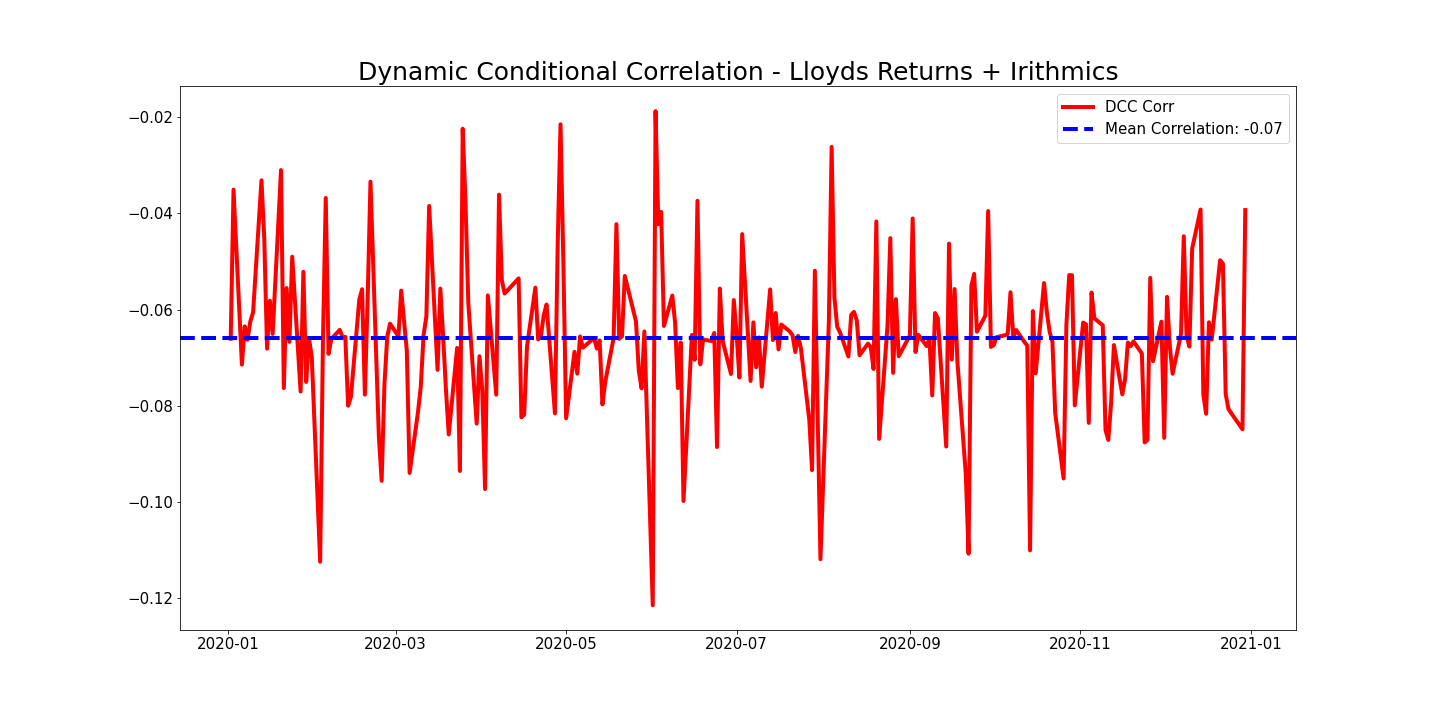
\includegraphics[scale = 0.30]{images/dcc/plot 1.png}
\caption{Lloyd's vs Irithmics DCC}
\label{fig: DCC Example}
\end{figure}

\subsubsection{Exogenous Covariate}
In order to include the Irithmics transformed probabilities as an exogenous covariate within the conditional volatility model, I decided it was more advantageous to implement the model using the Rugarch library in R \cite{rugarch}. This library allows for further specification within the model, to include a submodel hyperparameter of "external.regressors". I passed a matrix object, (in this case it is a univariate series so a nx1), which is included in the variance function when the model is fit. In order to keep the comparison between the empirical model with no regressors, and the new model including the probabilities, I ensured the only difference between the two was the newly included data. Shown in $\mathbf{Figure~4.8}$, the models fit the data using the training set up to the end of November (solid lines), and began the 1-day ahead rolling forecast using the out-of-sample test set (dashed lines). Because of the rigorous search for optimal hyperparameters in the univariate model, and the experimental constraints of keeping the same model there was no need to re-visit the grid search or selection criterion.  

\begin{figure}[H]
\centering
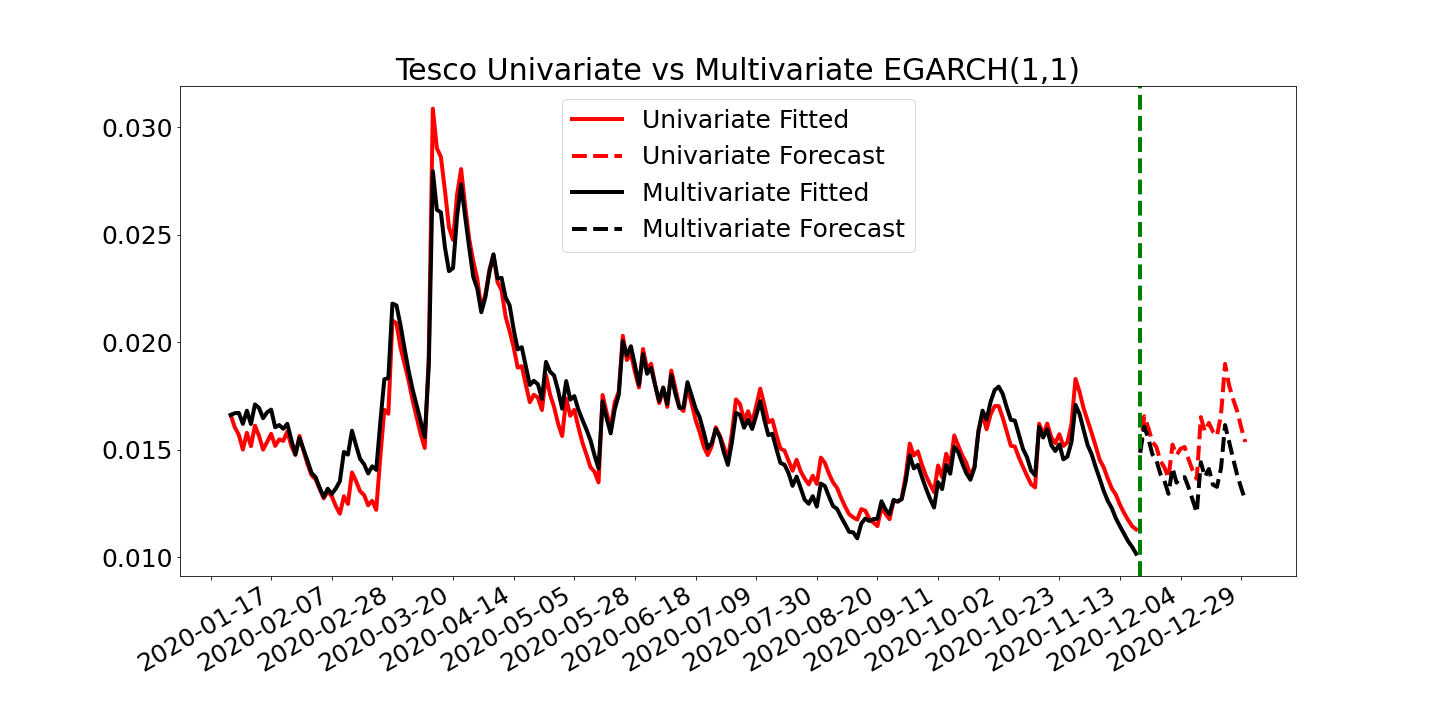
\includegraphics[scale = 0.30]{images/multiGarch/plot 2.png}
\caption{TESCO: Univariate vs Multivariate EGARCH(1,1)}
\label{fig: MV GARCH Example}
\end{figure}

\section{Model Validation}
While I did implement automated model selection methods, these are based on numeric criteria that do not necessarily address all components of a holistic research project. For each hyperparameter I included in my algorithm, I needed to validate the assumptions and limitations of including them in the model, as well as their relative impact on the forecast. 

\subsection{Residual Distributions}
The first hyperparameter I wanted to validate after viewing the grid search output tables was the residual distribution. It was very apparent that in the Tesco and Vodafone models, the students-t distribution was yielding lower values for AIC. I wanted to ensure not only was this accurate, but also there were no better available alternative distributions I could have used. $\mathbf{Figure~4.9}$ was a method used for my validation process, where I, similarly to the distribution of returns, I fit using maximum likelihood estimation, the standardized residuals to multiple distributions. For example, here it was clear why the students-t distribution was performing better than the normal distribution as there was more mass in the tails and a taller peak. I repeated this process with all four stocks optimal models to ensure validity in my residual hyperparameter decision.
\begin{figure}[H]
\centering
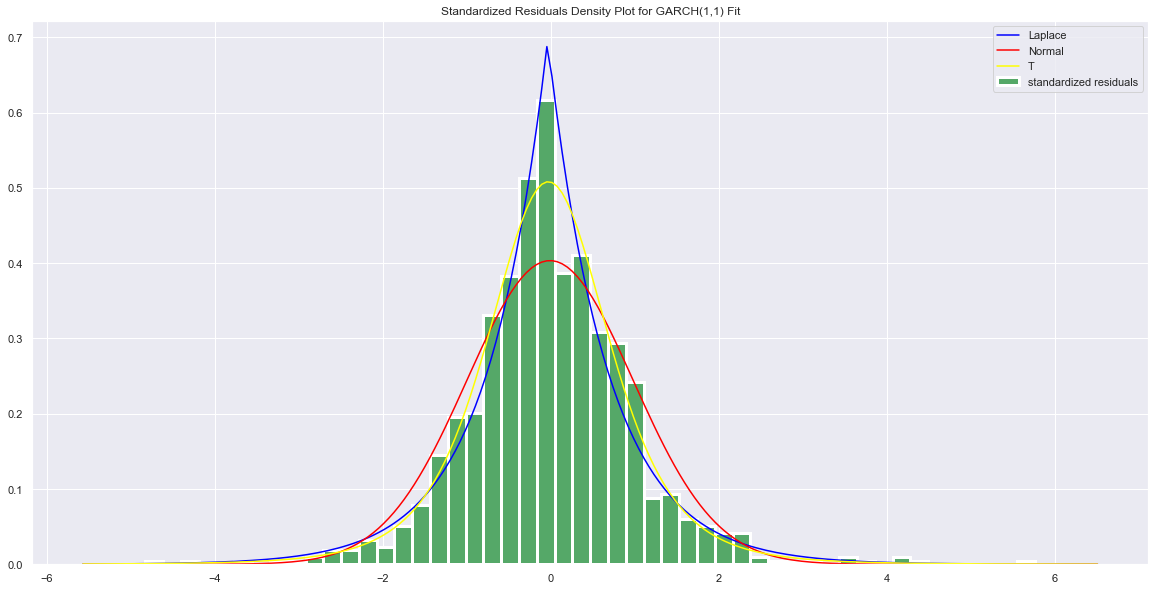
\includegraphics[scale = 0.35]{images/GarchResiduals.png}
\caption{GARCH(1,1) Residuals}
\label{fig: Garch Residuals}
\end{figure}

\subsection{Volatility Model}

I then evaluated why the different volatility models $\mathbf{(EGARCH~vs~GARCH)}$ faired differently. Different from the residual distribution, where a visual test was sufficient to gain understanding and confidence, the answer to this is was found through a better theoretical understanding of the $\mathbf{EGARCH}$ model. According to the creator of the $\mathbf{ARCH}$, Tim Bollserslev \cite{BOLLERSLEV1986307}, he now speaks on the EGARCH: "There is a stylized fact that the EGARCH model captures that is not contemplated by the GARCH model, which is the empirically observed fact that negative shocks at time t-1 have a stronger impact in the variance at time t than positive shocks" \cite{engle} Fundamentally, this concept builds on the older theory of a leverage effect found in a $\mathbf{GJR-GARCH}$. Engle further explained: "negative shock is $\gamma-\alpha$, while the effective coefficient associated with a positive shock is $\gamma+\alpha$. In financial time series, we generally find that $\gamma$ is negative and statistically significant" \cite{engle}. Fundamentally, the $\mathbf{EGARCH}$ model is able to capture the properties of market returns slightly better than the $\mathbf{GARCH}$, and Engle believes this is because the negative shocks have a larger and more significant affect on the next time periods variance than a positive shock. Intuitively this makes sense, as investor behavior tends to be more likely to sell a stock given bad news than buy an equal amount of stock given good news. Given this information I was comfortable with the results of the automated model selection.

\subsection{Lags (p,q)}

Finally, the evaluation of the lag parameters p and q were validated. I approached this problem in two ways, first was through the Partial Autocorrelation Function plots introduced in section one, evaluating the number of lags with significant autocorrelation $mathbf{Figure 4.4}$. This didn't necessarily give an indication of the number of lags the standard deviations had autocorrelation with, but it did give an indicator to the the autocorrelation between the actual time series observations. The second approach was to evaluate the significance of model parameters. In some cases the minimum AIC model would recommend a more complex model, say $\mathbf{EGARCH(3,2)}$, but the parameters for the coefficients of $\alpha_2,~\alpha_3,~\beta_2$ were not significant at the 0.05 level. There is also literature on the topic of models extending the general p=1,q=1 framework, such as Peter Hansen and Asger Lunde's \cite{Hansen11} which explained not only was the forecast accuracy showing no significant difference, but the model complexity actually hurt the analysis not helped. For this reason, whenever I saw a minimal difference in AIC, I always chose the simpler model.  

\subsection{Forecasting}
Since I am focusing on the 1-day ahead "Nowcast" I evaluated two forecasting methods: rolling window and fixed window. The rolling window has a fixed amount of days used in the model, ex: 100 day rolling the model starts on January 1st, uses 100 days of data and forecasts April 11th, the next forecast data begins on January 2nd uses data until April 11th and forecasts April 12th. Conversely, the expanding window forecast continues to aggregate data and the sample used to make the forecast gets larger with each step. An example of the difference in forecasts is shown in $\mathbf{Figure~4.10}$. For this portion of validation there was no objective "better" option, as both have strengths and weaknesses, so I decided to move forward with the forecast method yielding the least generalisation error.  
\begin{figure}[H]
\centering
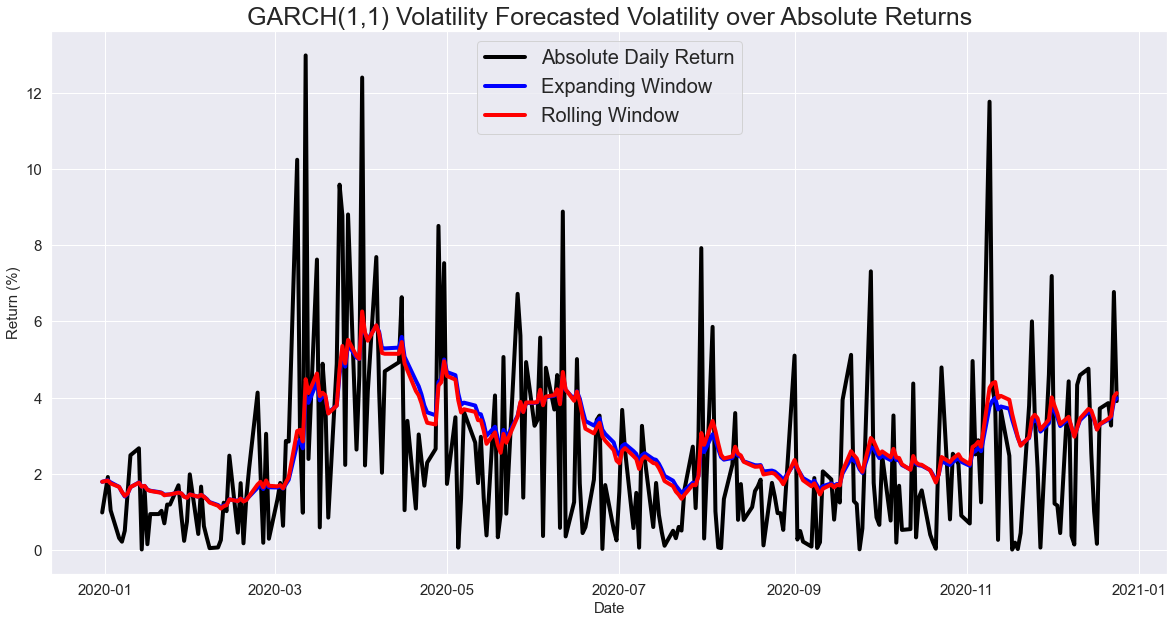
\includegraphics[scale = 0.35]{images/ForecastRollingExpanding1.png}
\caption{Rolling vs Expanding Forecast}
\label{fig: Fitting Plot}
\end{figure}

\section{Model Comparison}
Finally, I needed to determine a consistent method for comparing the accuracy of the forecasts. As noted prior, since it is not possible to extract the exact instantaneous standard deviation from the stock returns, a generally accepted proxy instead is the squared or absolute value of the selected returns, therefore I decided to compare the forecast conditional volatility to squared returns. The comparison was done using two metrics: Mean Absolute Error and Mean Squared Error.
$$
MAE~(Mean~Absolute~Error) = \sum|(\mathbf{X} - \mathbf{\hat{X}})
|$$ $$
MSE~(Mean~Squared~Error) = \sum(\mathbf{X} - \mathbf{\hat{X}})^2$$

The MAE and MSE simply give a generalisation error that can be compared across models to asses accuracy. These metrics will be used on the 1-day ahead rolling forecasts for the 25 day test dataset. 




\chapter{Results}
\label{ch:results}
\section{Univariate Model}
Using the grid search algorithm for automated model selection, each of the four stocks' returns yielded varying results. $\mathbf{Figure~5.1}$ shows the fitted model parameters for the two most optimal models, based on the minimization of the selected loss function: Akakie's Information Criterion (AIC). After the automated selection, I manually selected the model I would choose to implement based on significant parameters, model complexity, and residual distribution. As explained in $\mathbf{Section~4.3}$, there is more to a "best" model than the minimization of a loss function, so to ensure the best results I took a greater holistic approach to selection.

\subsection{Lloyd's}

The best models for Lloyds were \textbf{EGARCH(1,1), skewed-t}  \textbf{EGARCH(1,3),  skewed-t}. The two had negligible differences in AIC, but looking at the parameters, the added coefficients to the \textbf{(1,3)} model not only were insignificant, but it rendered the intercept and $\mathbf{\beta_1}$ coefficient insignificant as well (p-value $<$ 0.05). For this reason I chose the \textbf{EGARCH(1,1)} model, simpler and more significant parameters.

\subsection{Tesco}
The best models for Tesco were \textbf{EGARCH(1,2), students-t} and \textbf{EGARCH(2,1), students-t}. Model selection in this case was quite difficult, though the models themselves wouldn't produce overly different results. Both had 3 significant non-slope parameter, as well as the distribution parameter, while having insignificant intercepts. Because of the negligible difference in parameters, I defaulted to the automated model selection choice of  $\mathbf{EGARCH(1,2)~students-t}$ because of its minimum AIC value. 

\subsection{Rolls Royce}
The best models for Rolls Royce were \textbf{EGARCH(1,3), students-t} and \textbf{EGARCH(1,2), skewed-t}. The two had negligible differences in AIC, and no different in model coefficients (barring rounding error). The difference was the distribution of the residuals. To make a decision on which model, I fit using Maximum Likelihood Estimation the residuals to a distribution and found that again there was negligible difference. I chose the $\mathbf{EGARCH(1,3),~ students-t}$ model because it had the minimum AIC.  

\subsection{Vodafone}
The best models for Vodafone were \textbf{EGARCH(3,1), students-t} and \textbf{EGARCH(1,2), students-t}. The two had negligible differences in AIC, but looking at the parameters, the added coefficient to the (1,3) was not significant $\alpha_3$ and neither was $\omega$ the intercept. For this reason I chose the $\mathbf{EGARCH(1,2),~students-t}$ model, simpler and more significant parameters.  

\begin{figure}[hbt!]
\begin{subfigure}{.49\linewidth}
  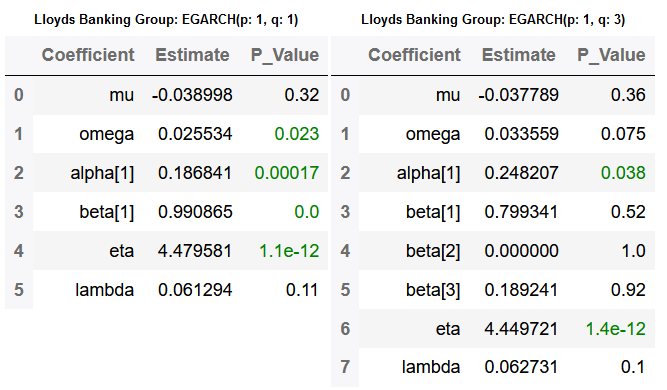
\includegraphics[width=\linewidth]{images/parameters/Lloy.png}
  \caption{LLOY}
  \label{fig:A}
\end{subfigure} % <-- "\hfill"
\begin{subfigure}{.49\linewidth}
  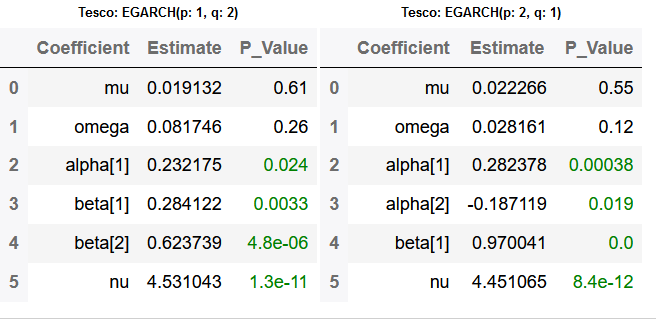
\includegraphics[width=\linewidth]{images/parameters/tesco.png}
  \caption{TSCO}
  \label{fig:B}
\end{subfigure}
\medskip % create some *vertical* separation between the graphs
\begin{subfigure}{.49\linewidth}
  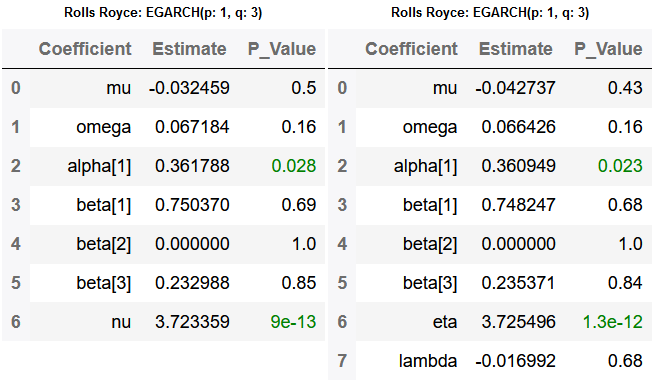
\includegraphics[width=\linewidth]{images/parameters/rr.png}
  \caption{RR}
  \label{fig:C}
\end{subfigure} % <-- "\hfill"
\begin{subfigure}{.49\linewidth}
  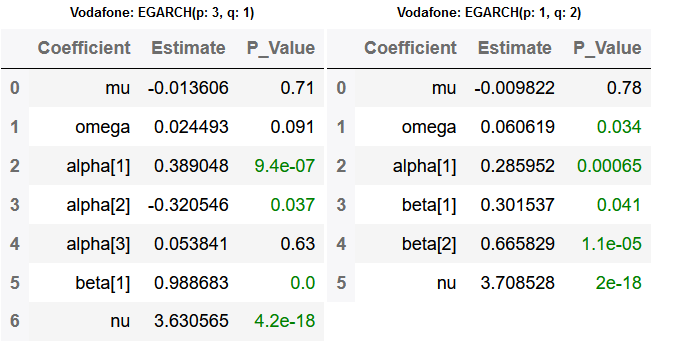
\includegraphics[width=\linewidth]{images/parameters/vod.png}
  \caption{VOD}
  \label{fig:D}
\end{subfigure}
\caption{Best Univariate Model Parameters}
\end{figure}

\subsection{Forecast Performance}
The resultant forecasts from these models yielded different results, and it became apparent that the fit and forecasts for Tesco and and Vodafone in both fixed and expanding window methodology were superior to that of Rolls Royce and Lloyd's. For the most accurate two models, the expanding window was more accurate than the fixed window. A great point of concern in the model fititng was the serious issues with the accuracy of the model for Rolls Royce returns, interestingly, the performance of the \textbf{EGARCH(1,3)} was worse than that of a model that simply took the mean of the information set's standard deviations. To interpret the table output, the scale of the chart was in \% so the best model, Vodafone, found itself within 2.21\% of the volatility proxy of squared centered returns on average. Though the models were simple, only including returns without any other information, a volatility forecast for 25 days with a mean absolute error of less than 2.4\% I believe to be very encouraging. For Tesco and Vodafone, the volatility forecasts are quite accurate and building complexity and information on top of these models could be quite advantageous. To continue work with Lloyd's and Rolls Royce, there is greater tuning to be done, these models are pretty much useless and should not be used moving forward.  
\begin{figure}[H]
\begin{subfigure}{.49\linewidth}
  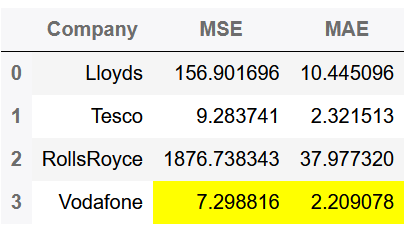
\includegraphics[width=\linewidth]{images/garchForecasts/expandingWindow.png}
  \caption{Expanding Window}
  \label{fig:A}
\end{subfigure} % <-- "\hfill"
\begin{subfigure}{.49\linewidth}
  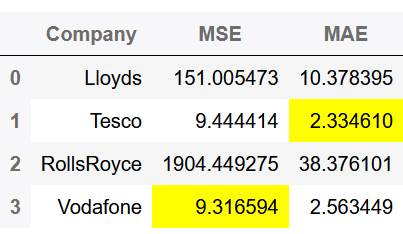
\includegraphics[width=\linewidth]{images/garchForecasts/fixedWindow.png}
  \caption{Fixed Window}
  \label{fig:B}
\end{subfigure}
\caption{Forecast Generalization Error}
\end{figure}

\section{Dynamic Conditional Correlation Model}
Implementing the DCC model on the model volatilities and the Irithmics conditional volatility did not immediately lead to a visualization or indication of any encouraging relationships between the Irithmics predicted short/sell probabilities and the stock returns. For the four stocks, the standard Pearson correlation coefficient between the two variables was about 0.07 - 0.09. Then using the dynamic model, I hoped to see if there were any events during the time series that there were significantly higher times of correlation, but unfortunately I never found this to be proven true. The highest correlated stock with Irithmics probabilities was Lloyd's, with its maximum conditional correlation was the beginning of February and June, but this value only reached 0.12. Ideally, this value would be much higher, as the next step in this analysis was to incorporate this value as an exogenous covariate implemented through linear regression. Theoretically all was not lost, as with financial applications any small fraction of increased accuracy can lead to large savings in a risk mitigation setting with investments, but greater correlation is obviously desired. To assist in the visualization over time, $\mathbf{Figure~5.3}$ plots the $\mathbf{EGARCH(1,1)}$ volatility with the Irithmics conditional volatility to show the linear relationship in a scatter plot and includes the sample correlation coefficient. Again, these results were not at all encouraging, but did not necessarily omit the prospect of slight increases in forecast accuracy by incorporating the exogenous data to the conditional volatility models \cite{DirtyQuant}. 


\begin{figure}[hbt!]
\begin{subfigure}{.49\linewidth}
  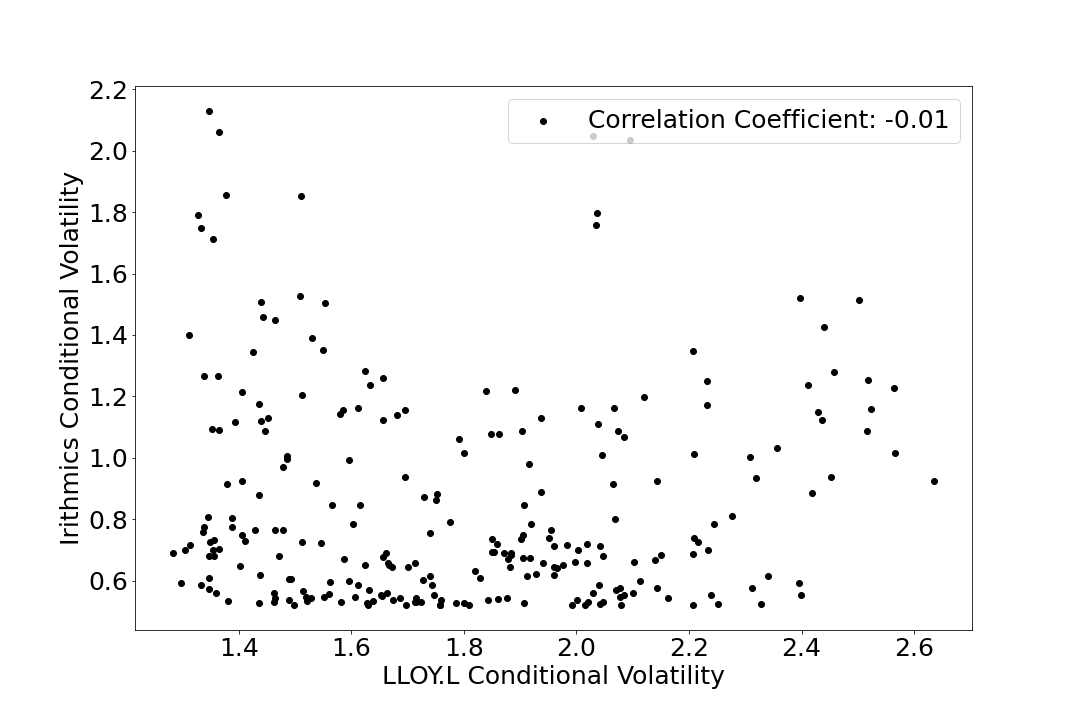
\includegraphics[width=\linewidth]{images/dcc_scatter/plot 1.png}
  \caption{LLOY}
  \label{fig:A}
\end{subfigure} % <-- "\hfill"
\begin{subfigure}{.49\linewidth}
  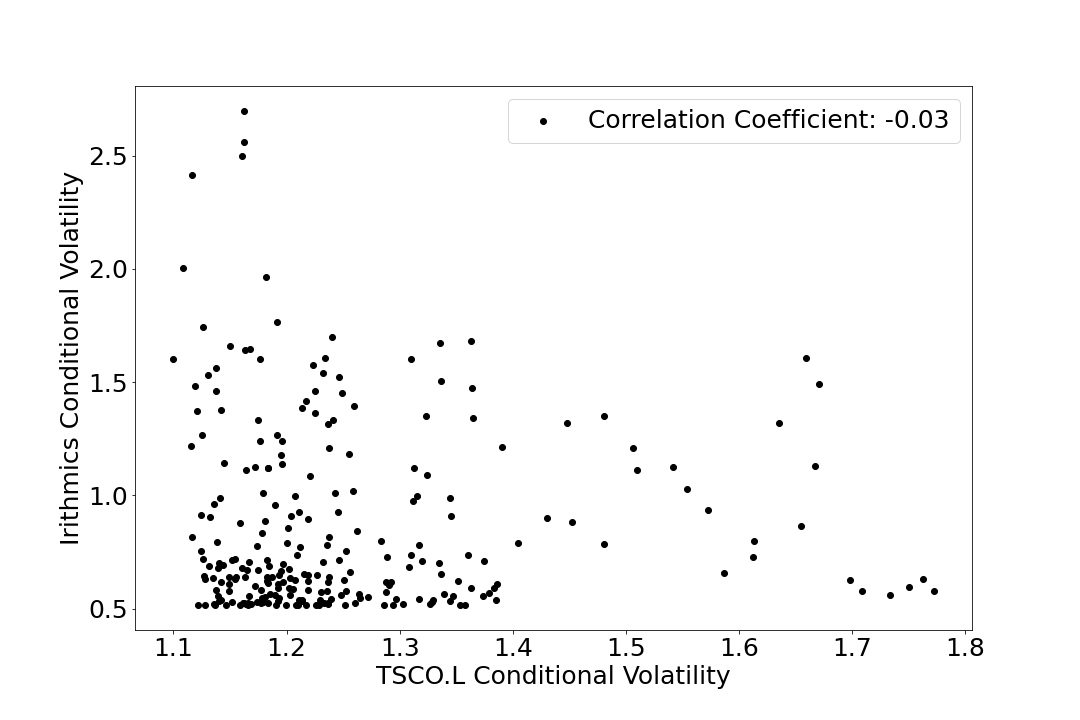
\includegraphics[width=\linewidth]{images/dcc_scatter/plot 2.png}
  \caption{TSCO}
  \label{fig:B}
\end{subfigure}
\medskip % create some *vertical* separation between the graphs
\begin{subfigure}{.49\linewidth}
  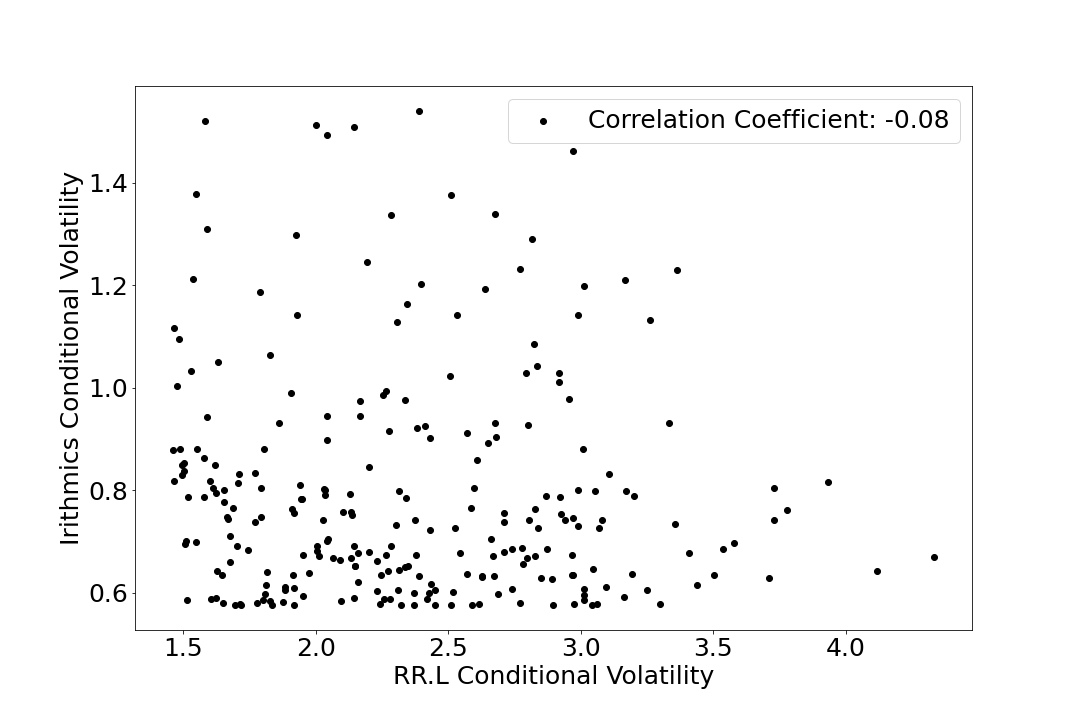
\includegraphics[width=\linewidth]{images/dcc_scatter/plot 3.png}
  \caption{RR}
  \label{fig:C}
\end{subfigure} % <-- "\hfill"
\begin{subfigure}{.49\linewidth}
  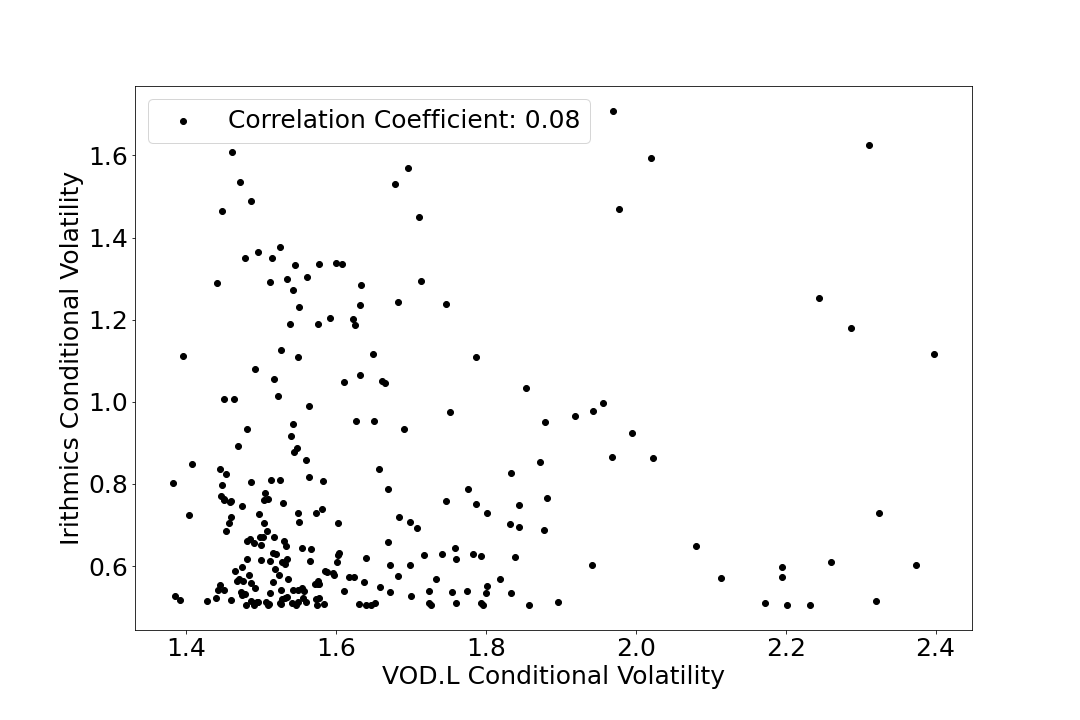
\includegraphics[width=\linewidth]{images/dcc_scatter/plot 4.png}
  \caption{VOD}
  \label{fig:D}
\end{subfigure}
\caption{DCC Scatter Plot}
\end{figure}

\section{Exogenous Covariate Model}
\subsection{Forecast Performance}
$\mathbf{Figure~5.4}$ highlights the comparative performance of the conditional volatility models forecasts with and without the exogenous covariate. 
\begin{figure}[H]
\centering
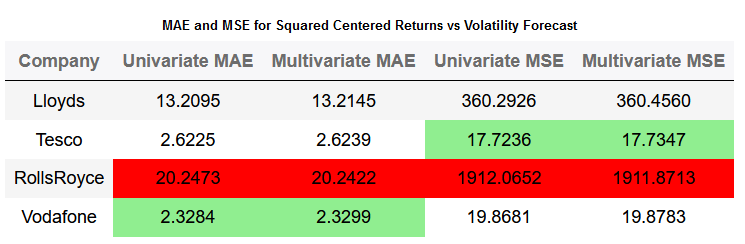
\includegraphics[scale=0.45]{images/multiGarch/GenErrorMSEMAE.png}
\caption{Multivariate Model Generalisation Error}
\label{fig: Multivariate Gen Error}
\end{figure}
Similar to what would be expected, given the information the Dynamic Conditional Correlation model results, there was no significant change to the model performance when incorporating the exogenous covariate of Irithmics data. In fact, though only by a very small amount, the model's performances were less accurate. The strongest models, Tesco and Vodafone, decreased in accuracy by a very insignificant factor of less than 0.001, and the worst performing models of Rolls Royce and Tesco had impacts slightly greater, but still less than 1\% different. $\mathbf{Figure~5.5}$ illustrates each models fitted values and rolling 1-day ahead nowcast. 
\begin{figure}[H]
\begin{subfigure}{.49\linewidth}
  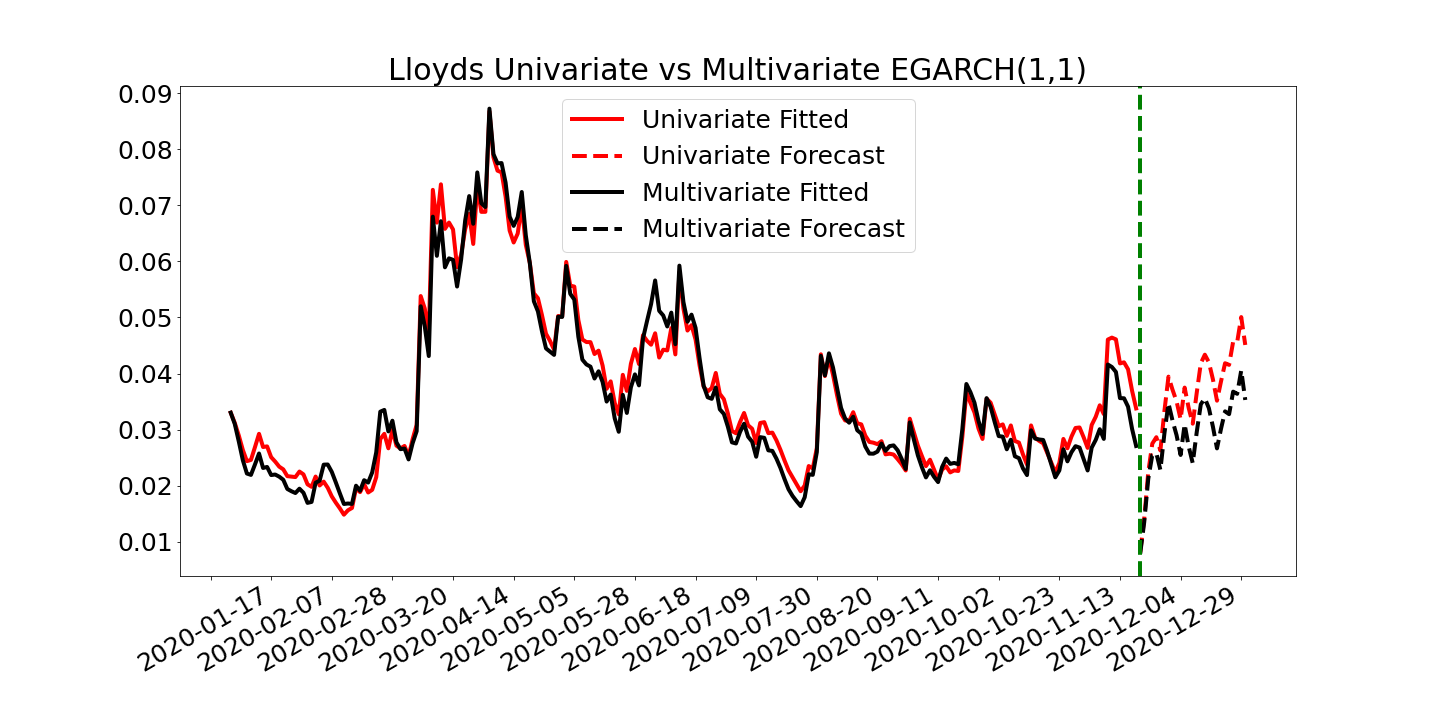
\includegraphics[width=\linewidth]{images/multiGarch/plot 1.png}
  \caption{LLOY}
  \label{fig:A}
\end{subfigure} % <-- "\hfill"
\begin{subfigure}{.49\linewidth}
  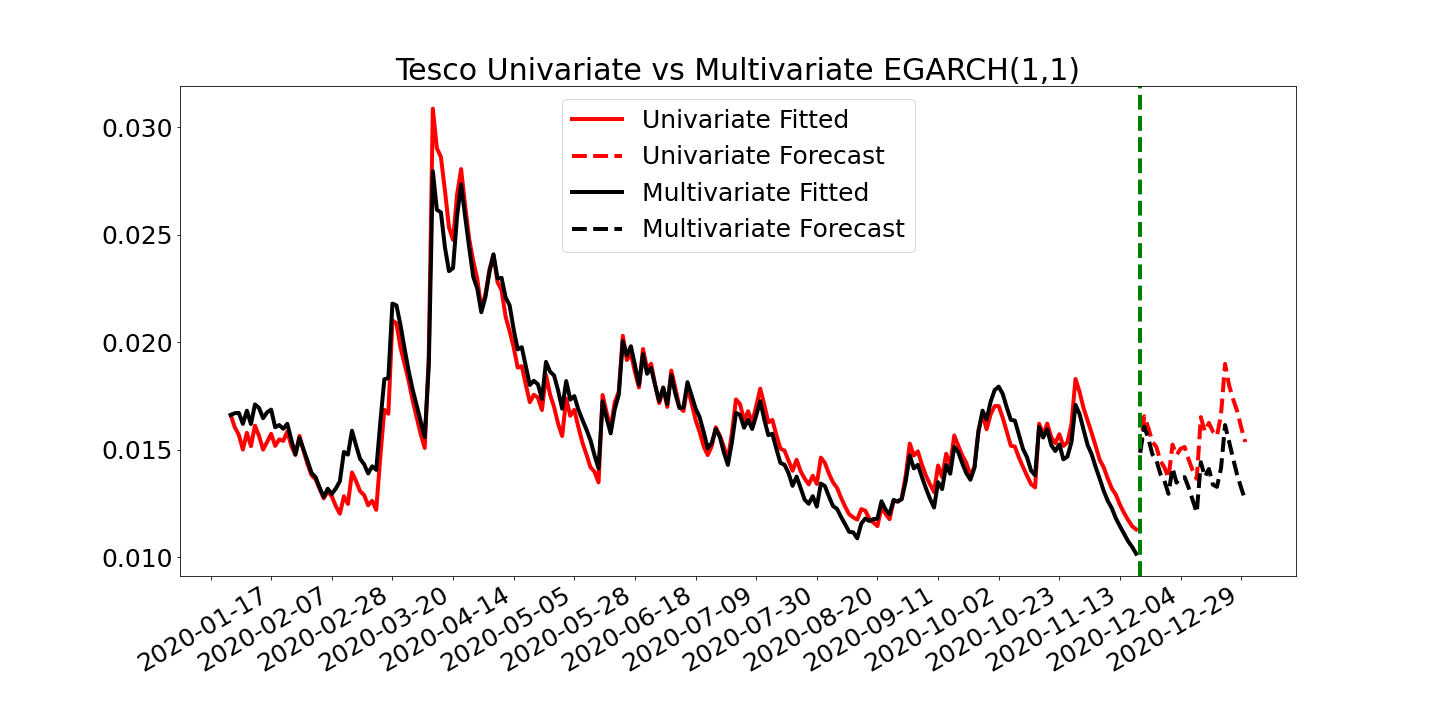
\includegraphics[width=\linewidth]{images/multiGarch/plot 2.png}
  \caption{TSCO}
  \label{fig:B}
\end{subfigure}
\medskip % create some *vertical* separation between the graphs
\begin{subfigure}{.49\linewidth}
  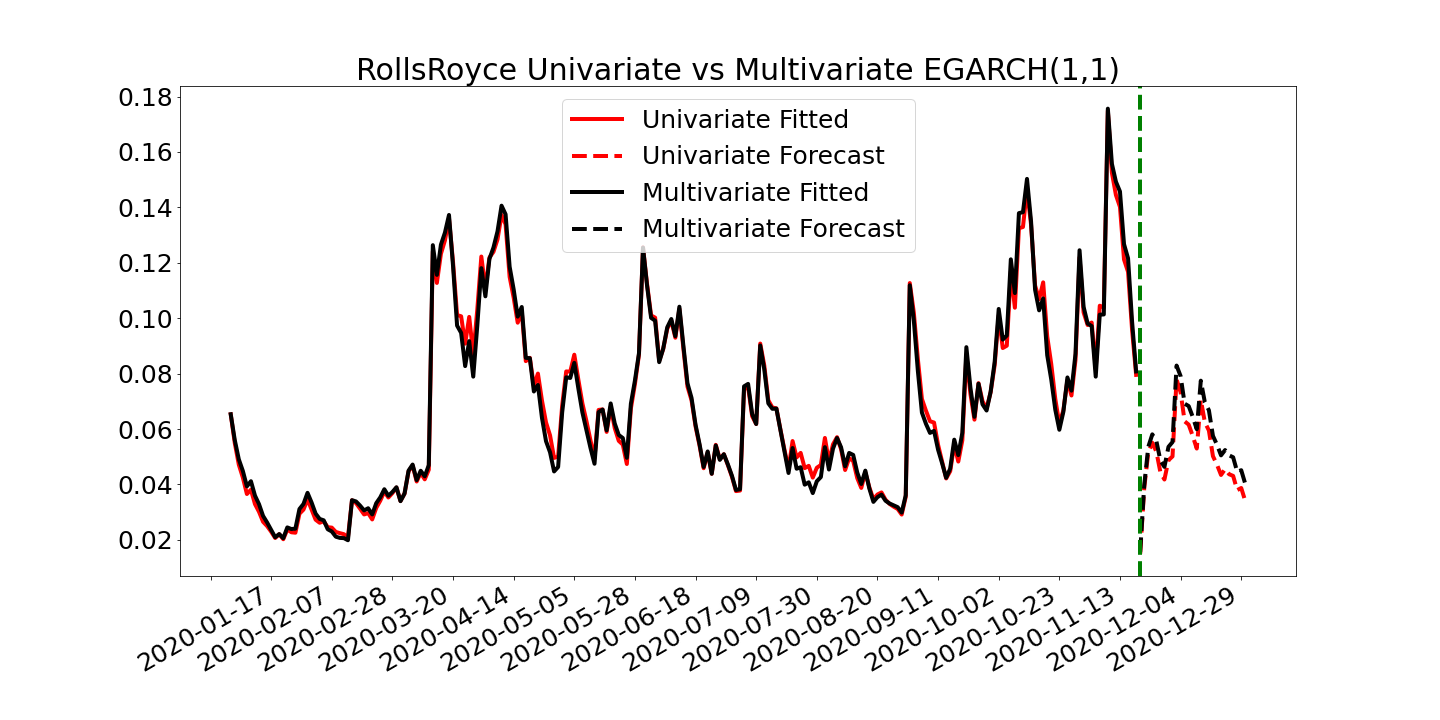
\includegraphics[width=\linewidth]{images/multiGarch/plot 3.png}
  \caption{RR}
  \label{fig:C}
\end{subfigure} % <-- "\hfill"
\begin{subfigure}{.49\linewidth}
  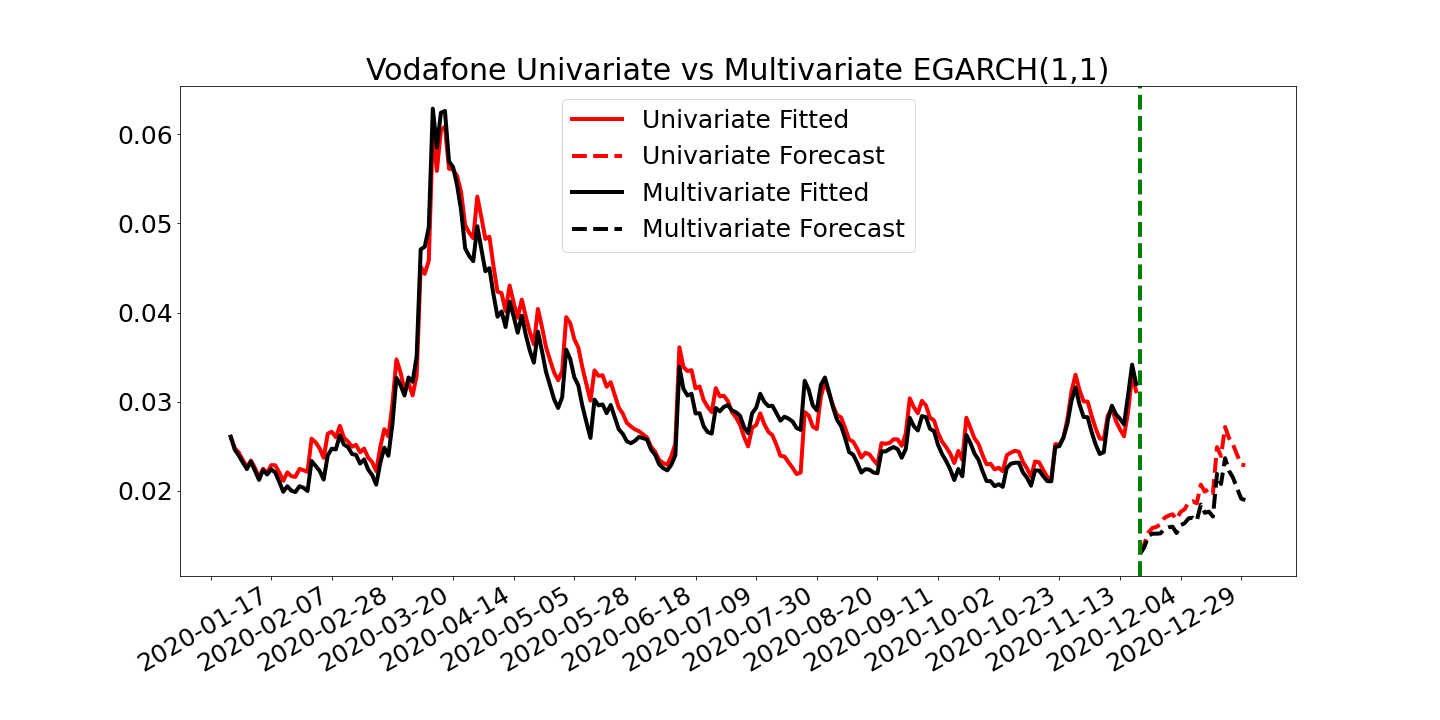
\includegraphics[width=\linewidth]{images/multiGarch/plot 4.png}
  \caption{VOD}
  \label{fig:D}
\end{subfigure}
\caption{Univariate vs Exogenous Forecasts}
\end{figure}

The intuitive interpretation of these results, is the Irithmics short probabilities, when incorporating into the volatility forecast acted almost exclusively as noise rather than signal of the data generating process. Looking closer at the fitted and forecast plots in \textbf{Figure (5.5)}, there are different intensities of impact the exogenous data has on the fitted and forecast values. Sub-figures b and d seem to show more extreme peaks and valleys in the univariate data vs the data incorporating the exogenous data, where sub-figures a and c track the univariate model near identically.
\chapter{Discussion}
\label{ch:Discussion}
\section{Overview}
In this dissertation, I set out to evaluate if a univariate conditional volatility forecast could be improved by adding an exogenous covariate to the already existing model. First, data was extracted from Yahoo Finance's database and transformed into continuous returns which were then modelled empirically using grid-search selected $\mathbf{EGARCH}$ models. Then, after receiving Irithmic's data provided, these data were transformed via the weight decaying algorithm. Once the data processing was complete, I trained the optimal models and forecasted and compared outputs. Following the univariate modelling, I implemented a Dynamic Conditional Correlation model to evaluate the relationship between the selected exogenous covariate and the modelled conditional volatility. Though yielding mediocre results, I continued with the final process of fitting an $\mathbf{EGARCH}$ model with an exogenous covariate. Disappointingly, the results of the model were not improved, though a greater understanding of conditional volatility modelling, exogenous data model integration, and many ideas for future work were derived. This project approached a well researched area of volatility modelling, with a novel approach of taking a tangentially related piece of non-standard data, standardizing the format in a generalisible fashion and implemented it using empirical methods.  


\section{Future Work}
There is great opportunity for further work on this topic. First, I think there is great potential for further incorporating exogenous variables to conditional volatility forecasts. There is research in the area, but has plenty of room for continued work. I think incorporating linear and non-linear models as an extension to $\mathbf{EGARCH}$ models could be very powerful. Of course there is the balance in statistics between interpretation and prediction, but if one is trying to simply improve forecast accuracy, finding exogenous data sets (could be very large data) to accompany the empirical model could be very powerful. I also think there is opportunity for great model improvements using the Dynamic Conditional Correlation models in a similar study. Given the constraints, I was only able to implement it once, but the possibility for incorporating more data such as interest rates, the FTSE 100 index, or an aggregate of the sector the targeted stock is in. Second, I believe there is much greater opportunity to explore avenues to more effectively use the Irithmics data. Though it was not proved in this project, the power of the Wisdom of the Crowds cannot be understated. Having information about the predicted behavior of trillion's of pounds of assets moving in Britain has many use cases beyond just volatility predictions. I believe a possible greater aggregation of the data across the entire FTSE 100, rather than a selected group of stocks could yield better results, as the greater grouping could smooth out anomalies and increase predictability. Lastly, there is great room to contribute to the Python and R time series open source community. As the research transcends traditional models, there is great opportunity to contribute to development of time series modelling libraries of greater complexity (rugarch in R, arch in Python). I have greatly enjoyed the artistry of programming and developing models and am greatly excited by the opportunity to contribute further to the literature in Financial Time Series. 

\section{Limitations}
As this research completed for an M.Sc. Dissertation, there were limitations to completing a fruitful study. Firstly was the datset size. As Irithmics graciously donated these data free of charge, to explore a novel concept, I did not have 1000's trading day history for each stock, instead about 252. This lead to challenges in fitting and training a model with holdout data for out of sample testing, to identify generalization error and tune hyperparameters, while balancing the amount of data for a large sample to train with, though this can also be attributed to the challenges of working with time series data. For example, traditional methods for training neural networks or tree models like bootstrapping or k-fold cross validation are not available as testing data outside the temporal constraint is not useful. Second, the constraint of time. Given this project was completed in 2-3 months, I had to make decisions and pursue ideas very quickly and there was no time to restart or take a step back, read full textbooks and many papers. Lastly, the constraint of the exogenous data itself. The Irithmics data is the corporation's proprietary models prediction of what the aggregate decision of the funds to short/sell a stock. The maximum probability was about 0.07, so even if 7\% of the 250,000 funds decided they would sell the stock, depending on the individual portfolio weights, and actions of other institutions, macroeconomic events and other investors, there was no reason to say this will increase the instantaneous volatility of the stock on that day.  




\newpage
\frontpagestyle
\bibliographystyle{apalike}
\renewcommand\bibname{Bibliography}
\bibliography{bibliography/bibliography}
\addcontentsline{toc}{chapter}{Bibliography}



    \renewcommand{\listfigurename}{Selected Figures}
    %\renewcommand{\listtablename}{Glossary of Terms}
    
    %\cleardoublepage
    %\listoftables
    %\addstarredchapter{Glossary of Terms}
    %\chaptermark{Glossary of Terms}
    %\pagestyle{plain}
    

    \cleardoublepage
    \addstarredchapter{Figures}
    \chaptermark{Figures}
    \listoffigures
    \pagestyle{plain}
    
    %\cleardoublepage
   %\printnoidxglossary[type=\acronymtype,style=index,nonumberlist,title=Abbreviations, nogroupskip=true]
    %\printnoidxglossary[title=Nomenclature]
    %\addstarredchapter{Glossary of Terms}
    %\chaptermark{Abbreviations}
    %\pagestyle{plain}
\chapter*{Appendix}
\label{ch:Appendix}
\section*{Python \& R Code}
I used a mixture of Python and R code to exploit the strengths of each language. Specifically I found R to be more useful for data processing, as the tidyverse allows similar commands to a SQL environment, as well as rugarch for incorporating exogenous variables.   
Code can be found on the following pages: 
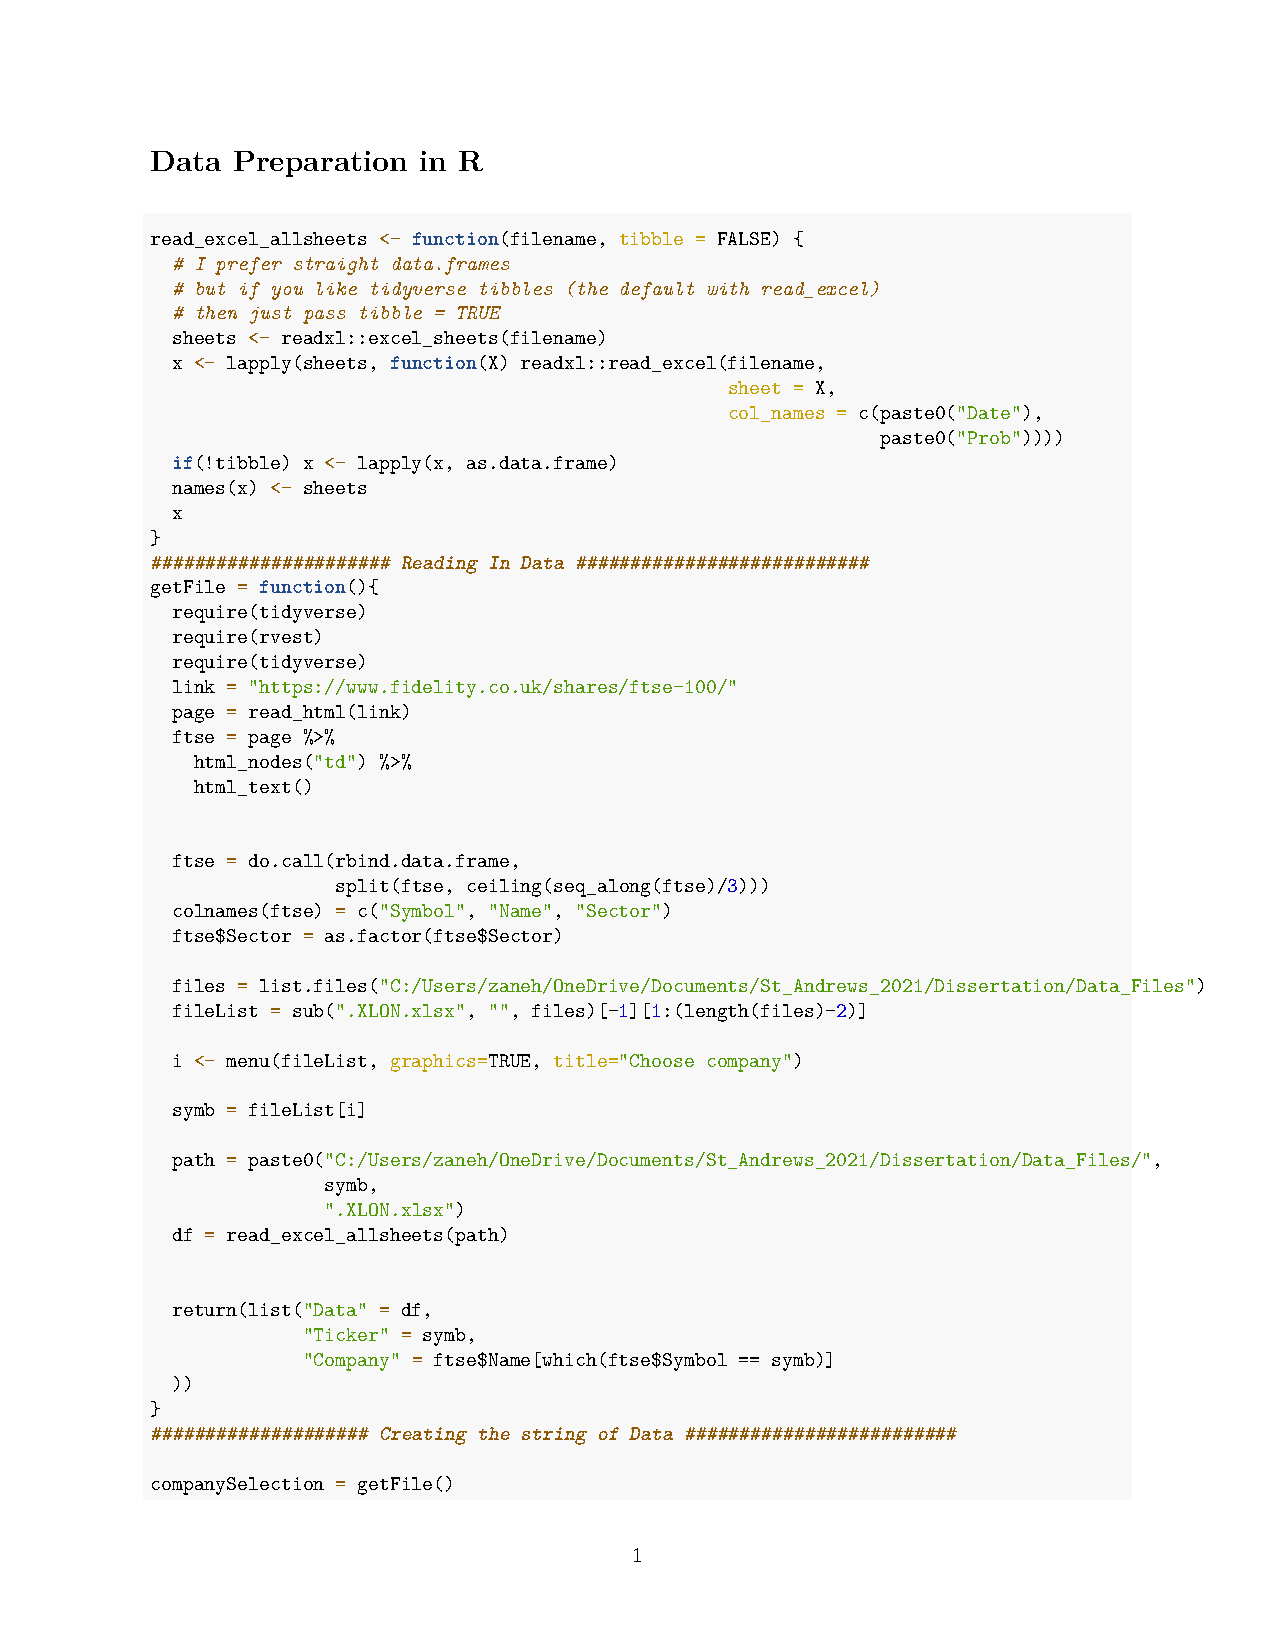
\includepdf[pages=-]{appendices/PDFs/Dissertation_Code.pdf}
\addcontentsline{toc}{chapter}{Appendix}




\end{document}